\chapter{Methods}
This chapter describes the basic principles and strategies used to achieve the project objectives. 
\section{Software}
%\textit{Hér skrifa ég hvað ég notaði og hvernig og referenca í undirkafla í hvert skipti}

This chapter includes a brief overview of the software that was used in this project. The main software programming language will be Python version 2.7 \cite{noauthor_python_nodate}, since that is a version that the school computer has. ROS will be used to communicate between nodes and programs, the ROS distribution version will be the \textit{ROS Melodic Morenia}\cite{noauthor_melodic_nodate}. In \textit{Figure \ref{fig:roswork}} shows the ROS setup in a flowchart that shows how the nodes communicate in this project.
\begin{figure}[h]
    \centering
    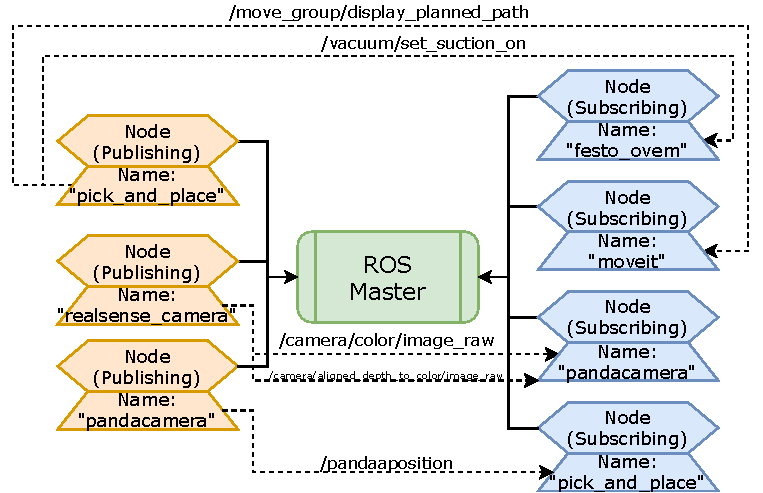
\includegraphics[width=0.7\textwidth]{graphics/ros.pdf}
    \caption{ROS setup}
    \label{fig:roswork}
\end{figure}

%The main hardware parts will be explained in several subsections: robot manipulator (\ref{subsec:robot}), robot end effector (\ref{subsec:robotend}) and a camera (\ref{subsec:camera}). 

\subsection{Data Annotation}
COCO Annotator is a web-based image annotation application that allows you to mark up images rapidly and conveniently to create training data for image localization and object detection. It has a variety of unique features, such as the ability to label an image segment, monitor object instances, label objects with disconnected visible sections, and store and export annotations in the well-known COCO format. An intuitive and customizable interface guides you through the annotation process, which includes a range of resources for constructing accurate datasets \cite{brooks_jsbrokscoco-annotator_2021}.
% \begin{figure}[h]
%     \centering
%     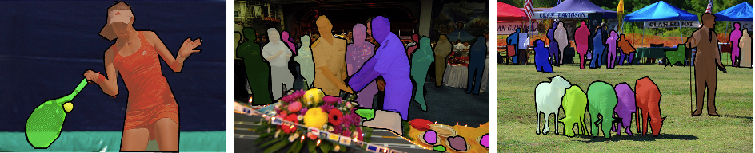
\includegraphics[width=1\textwidth]{graphics/coco.png}
%     \caption{An example of how images are annotated by hand}
%     \label{fig:coco}
% \end{figure}
% \linespread{0}

\subsection{Object detection}


You only look once (YOLO) is a real-time object detection system that is at the cutting edge of technology. 
It was first developed by Josep Redmon a neural network architecture.
Object identification, classification, and localization are all performed in a single network pass with YOLO. 
As a result, it is more computationally efficient and robust than other networks that only perform one or two of these tasks at the same time. 
With the help of dimension clusters, YOLO predicts bounding boxes (convolutional neural network). 
It's so computationally powerful that it can operate on a live image stream, which comes in handy when operating on a robot in real time \cite{redmon_yolov3_2018}.
\begin{figure} [ht]
    \centering
    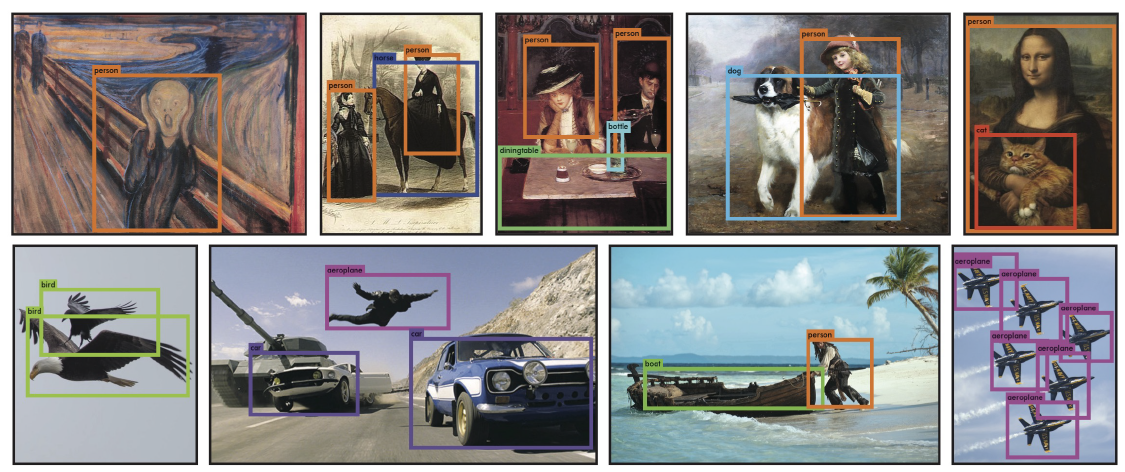
\includegraphics[width = 0.75 \textwidth]{graphics/yolo.PNG}
    \caption{You Only Look Once: Unified, Real-Time Object Detection \cite{redmon_you_2016}}
    \label{fig:yolo}
\end{figure}


In this project \textit{YOLOv4}\cite{bochkovskiy_yolov4_2020} algorithm was used to detect objects in the bin and mark a rectangle around them. 
YOLO algorithm was chosen since it is easy to use and the major advantage of YOLO is its excellent speed, it also understands the general representation of objects. YOLO algorithm outperforms other detection algorithms, including \textit{Deformable Parts Model(DPM)} and \textit{R-CNN}, when generalizing natural pictures from artworks to other fields.

%When the YOLO has found an object with high accuracy it sends to the robot coordinates of the center point, and then there is possible to get the depth from the camera.

% \begin{figure}[h]
%     \centering
%     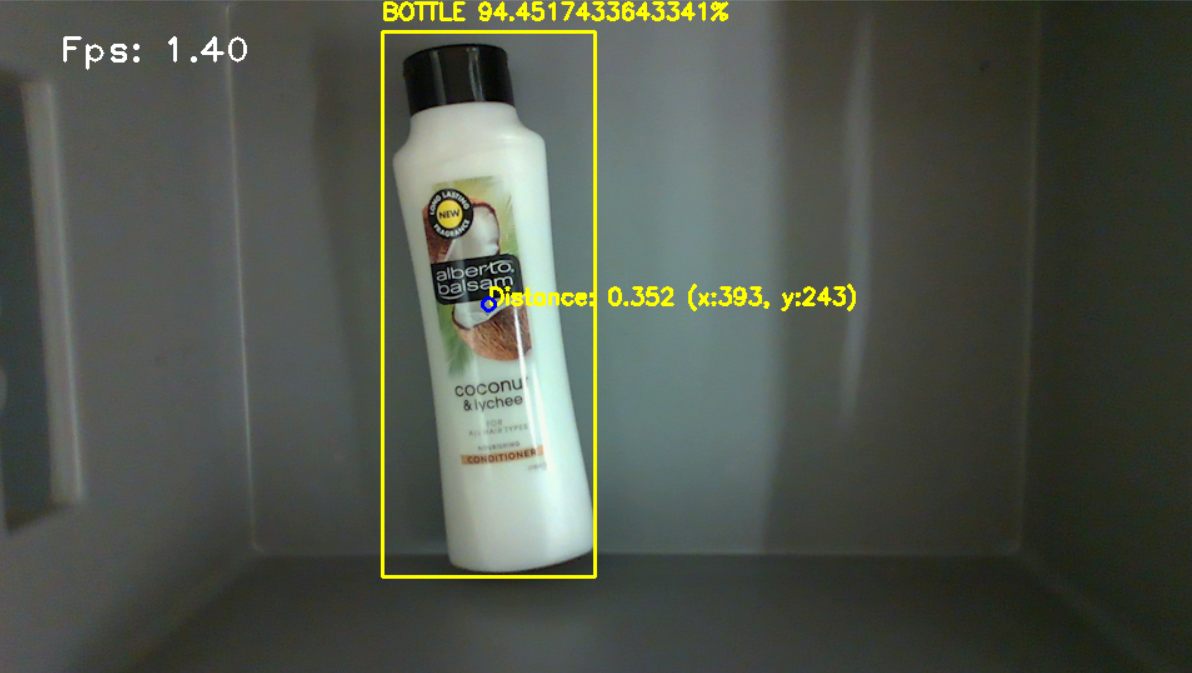
\includegraphics[width=0.4\textwidth]{graphics/detectandmeasure.PNG}
%     \caption{Here is an example of an YOLO detect application}
%     \label{fig:yolodetect}
% \end{figure}

\subsection{OpenCV}
OpenCV is a cross-platform library that allows one to build real-time computer vision applications. It is primarily concerned with image recognition, video capturing, and interpretation, with features such as face detection and object detection. OpenCV is a free and open-source library of programming functions primarily for real-time computer vision \cite{noauthor_opencv_nodate}.

One of OpenCV's aims is to provide an easy-to-use computer vision infrastructure that allows people to easily create fairly complex vision applications. Over 500 functions in the OpenCV library cover a wide range of vision applications, including factory product inspection, medical imaging, security, user interface, camera calibration, stereo vision, and robotics. Since computer vision and machine learning often go hand in hand, OpenCV includes a comprehensive, general-purpose Machine Learning library \cite{kaehler_what_2016}.

\begin{figure}[h]
    \centering
    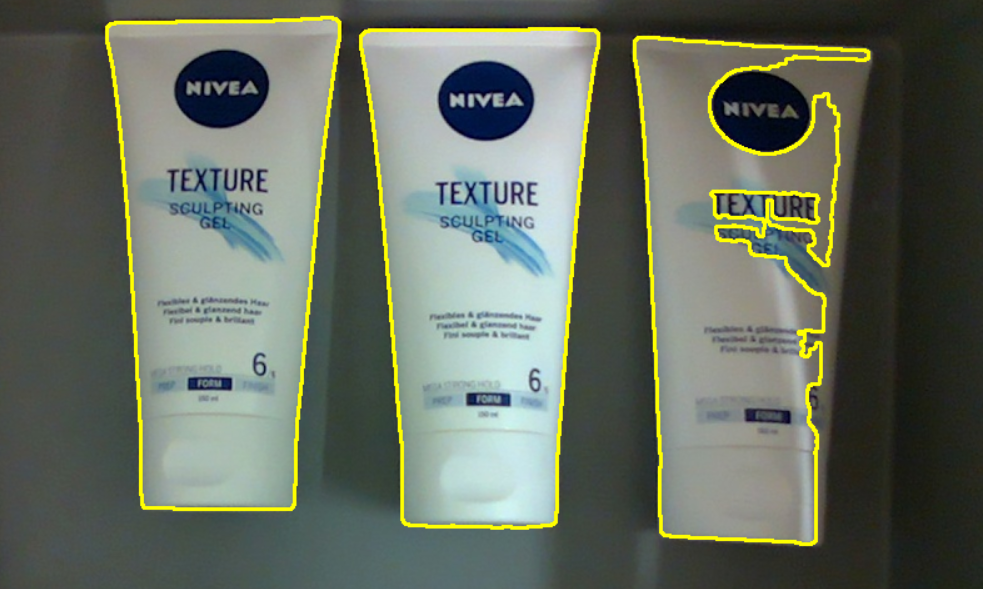
\includegraphics[width=0.65\textwidth]{graphics/contour.PNG}
    \caption{An example of how OpenCV can find contours}
    \label{fig:opencvcontour}
\end{figure}

OpenCV was used in this project to work on images from the camera, the main functions that were used in this project were \textit{structural simularity} to compute the difference between two images,  \textit{threshold} to threshold the difference image followed by finding contours to obtain the regions of the two input images that differ and then the \textit{findContours} function to find the contours, draw around the objects and measure the objects.

\clearpage
\section{Hardware \label{sec:hardware}}
%\ifdraft{\textit{Hér skrifa ég hvað ég notaði og hvernig og referenca í undirkafla í hvert skipti (Má lesa yfir\\}}
This chapter includes a brief overview of the hardware that was used in this project. The main hardware parts will be explained in several subsections: robot manipulator \textit{(Sec:\ref{subsec:robot})}, robot end effector \textit{(Sec:\ref{subsec:robotend})} and a camera \textit{(Sec:\ref{subsec:camera})}. The setup can been seen in \textit{Figure \ref{fig:setupproject}}.

\begin{figure}[h]
    \centering
    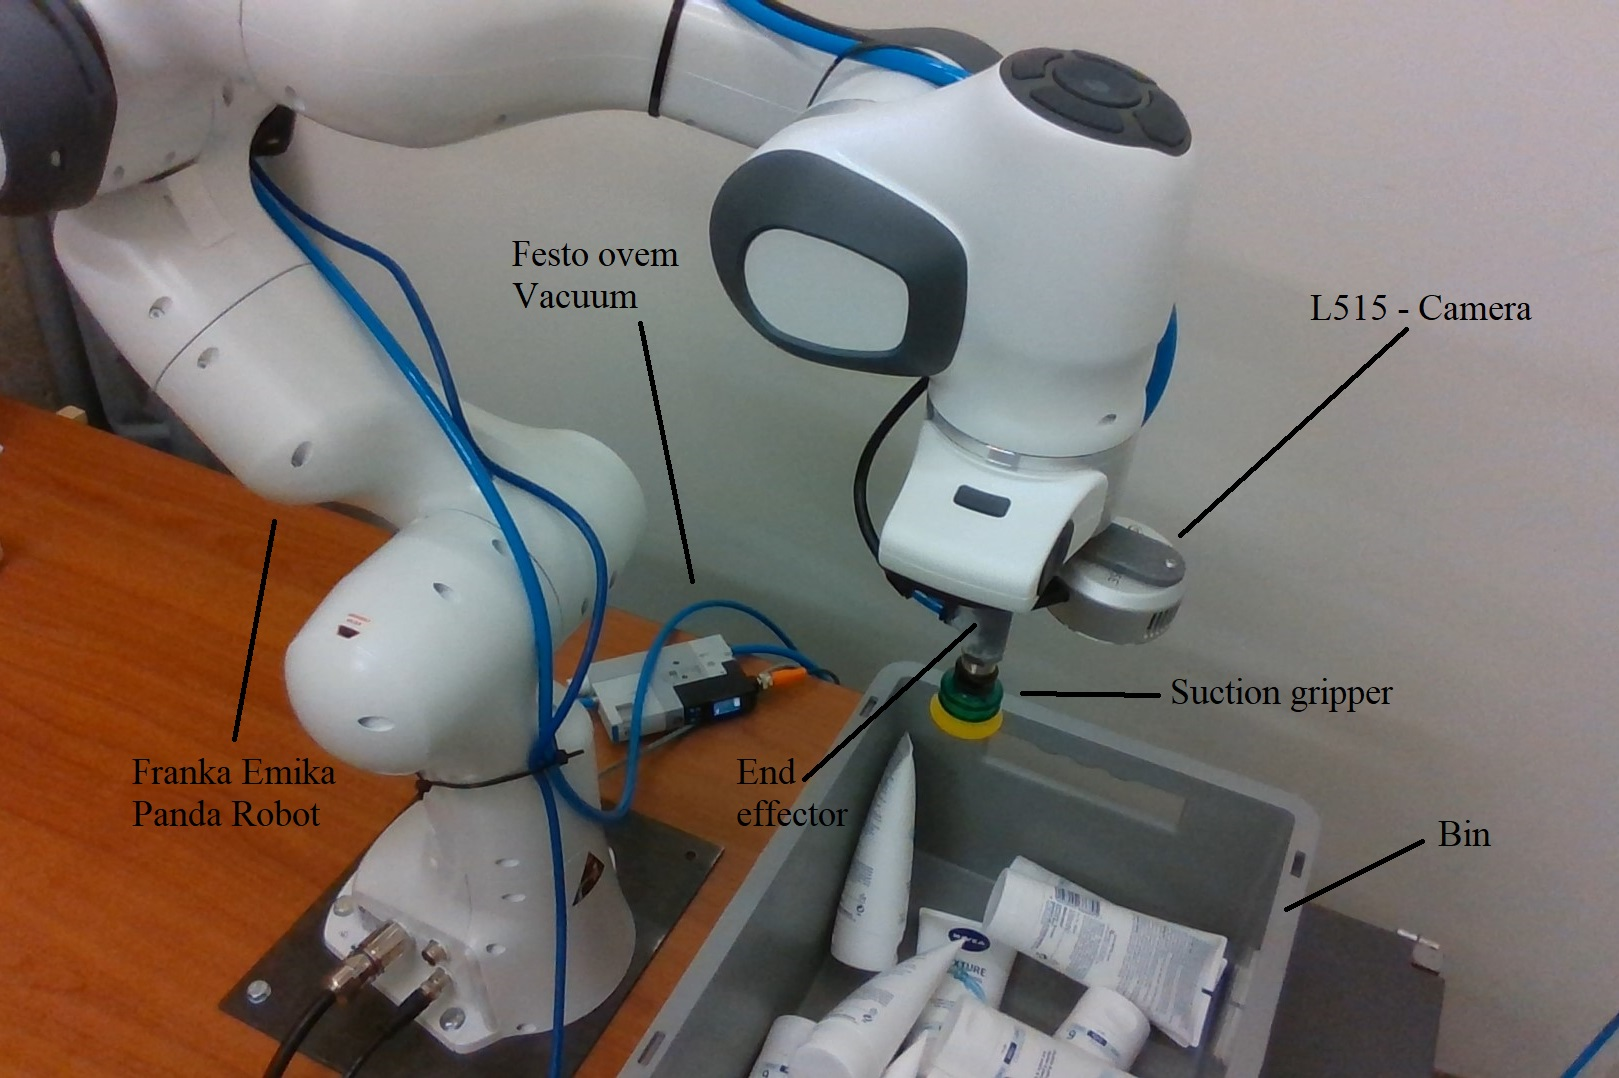
\includegraphics[width = 0.65\textwidth]{graphics/setup.jpg}
    \caption{The hardware setup for this project}
    \label{fig:setupproject}
\end{figure}
\linespread{0}
\subsection{PC cores}
\vspace{0.8cm}
\subsubsection*{Training neural networks}
The GPU for training neural networks will be the \textit{NVIDIA GeForce RTX 2080 Ti}\cite{noauthor_graphics_nodate}.
A GPU is nearly necessary to train neural networks. The GeForce RTX 2080 Ti is a budget-friendly option for the dense system configuration with a blower size. Titan RTX, Tesla V100, Titan V, GTX 1080 Ti, and Titan Xp provide the best price versus performance. Its performance at training neural networks is close to Tesla V100 speed, which is one of the world's most powerful GPU\cite{noauthor_deep_2018}. 

\subsubsection*{Computer to control the robot}
The computer that will be used in this project to control the robot is a \textit{Lenovo ThinkCentre M83 SFF Pro Desktop}\cite{noauthor_thinkcentre_nodate} computer, it was chosen since it has ROS and had already been used to program the Franka Emika robot. 

\clearpage

\subsection{Robot manipulator\label{subsec:robot}}
The Robot manipulator that was used in this project is a Franka Emika Panda robot and was chosen because the RU (Reykjavik University) owns a robot of that type. Franka Emika Panda is a Cobot that has 7 working axes with torque sensors in all 7 axes \cite{gmbh_franka_nodate}. Panda includes the characteristics of a conventional stiff industrial robot with a repeatability of +/- 0.1 mm even at elevated velocities of up to 2 m/s with a negligible direction variance. This enables accurate, resilient, and quick manufacturing method execution. 
% \begin{figure}[h]
%     \centering
%     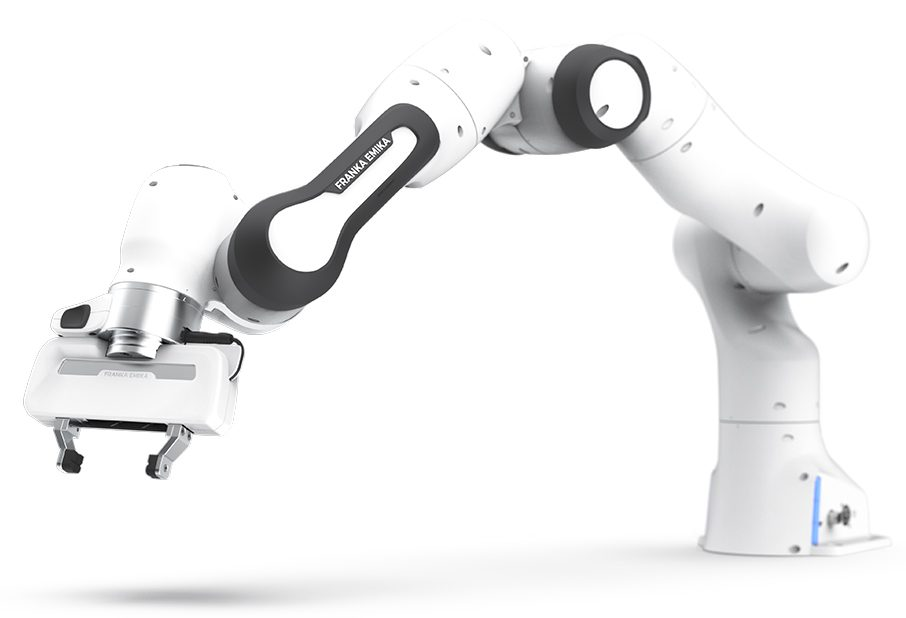
\includegraphics[width=0.8\textwidth]{graphics/frankapanda.jpg}
%     \caption{Franka Emika Panda}
%     \label{fig:frankaemika}
% \end{figure}
\begin{figure}[h]
    \centering
    % include first image
    \subfloat[Franka Emika Panda ]{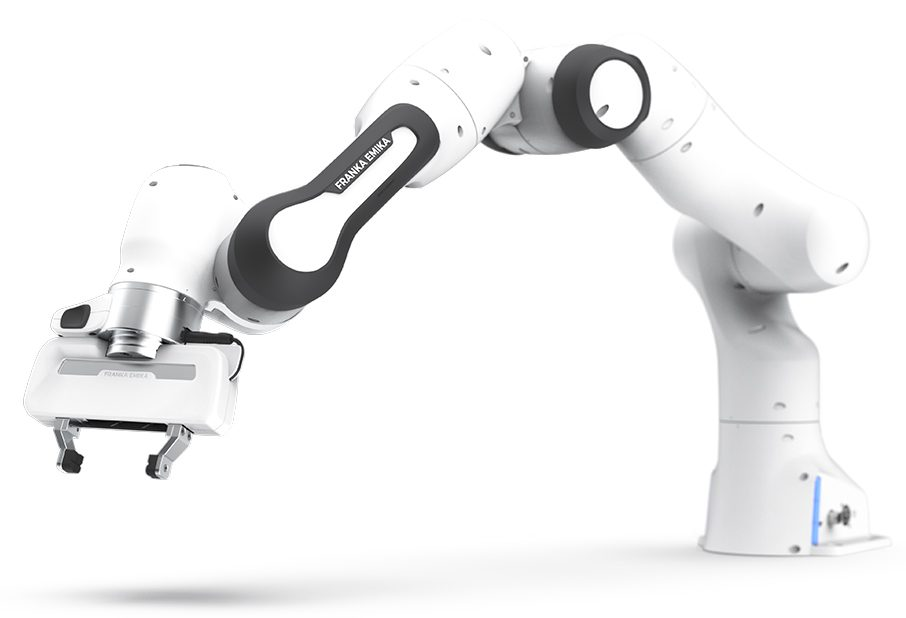
\includegraphics[width=0.6\textwidth]{graphics/frankapanda.jpg}}
    \hfill
    \subfloat[Franka Emika Panda setup]{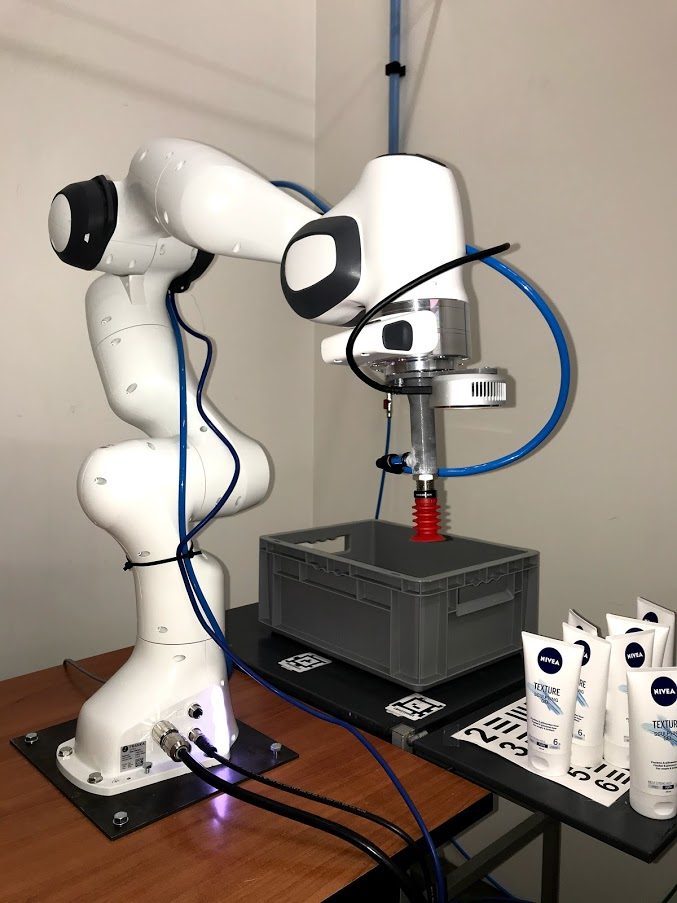
\includegraphics[width=0.35\textwidth]{graphics/pandarobot.jpg}}
    \caption{Robot manipulator}
    \label{figure: frankaemika}
\end{figure}
% Má eyða seinna\begin{itemize}
%     \item \url{https://www.franka.de/}
%     \item Franka Emika Panda in Gazebo with ROS and Docker \cite{wallkotter_franka_2020}
% \end{itemize}

\subsection{Robot end effector\label{subsec:robotend}}
A peripheral device that connects to a robot's wrist and allows it to communicate with its mission is known as an end effector. Grippers, process tools, and sensors are all examples of end effectors, which are mechanical or electromechanical \cite{wilson_relative_1996}. 

In this case a suction gripper was used. It was designed in Autodesk Inventor \cite{noauthor_inventor_nodate} and 3D printed in TEVO Nereus 3D printer that Reykjavik University owns. At the end of the effector there is a suction cup connected to Festo Vacuum generator OVEM with an 8mm tube.
\begin{figure}[ht]
    \centering
    % include first image
    \subfloat[Inventor drawing ]{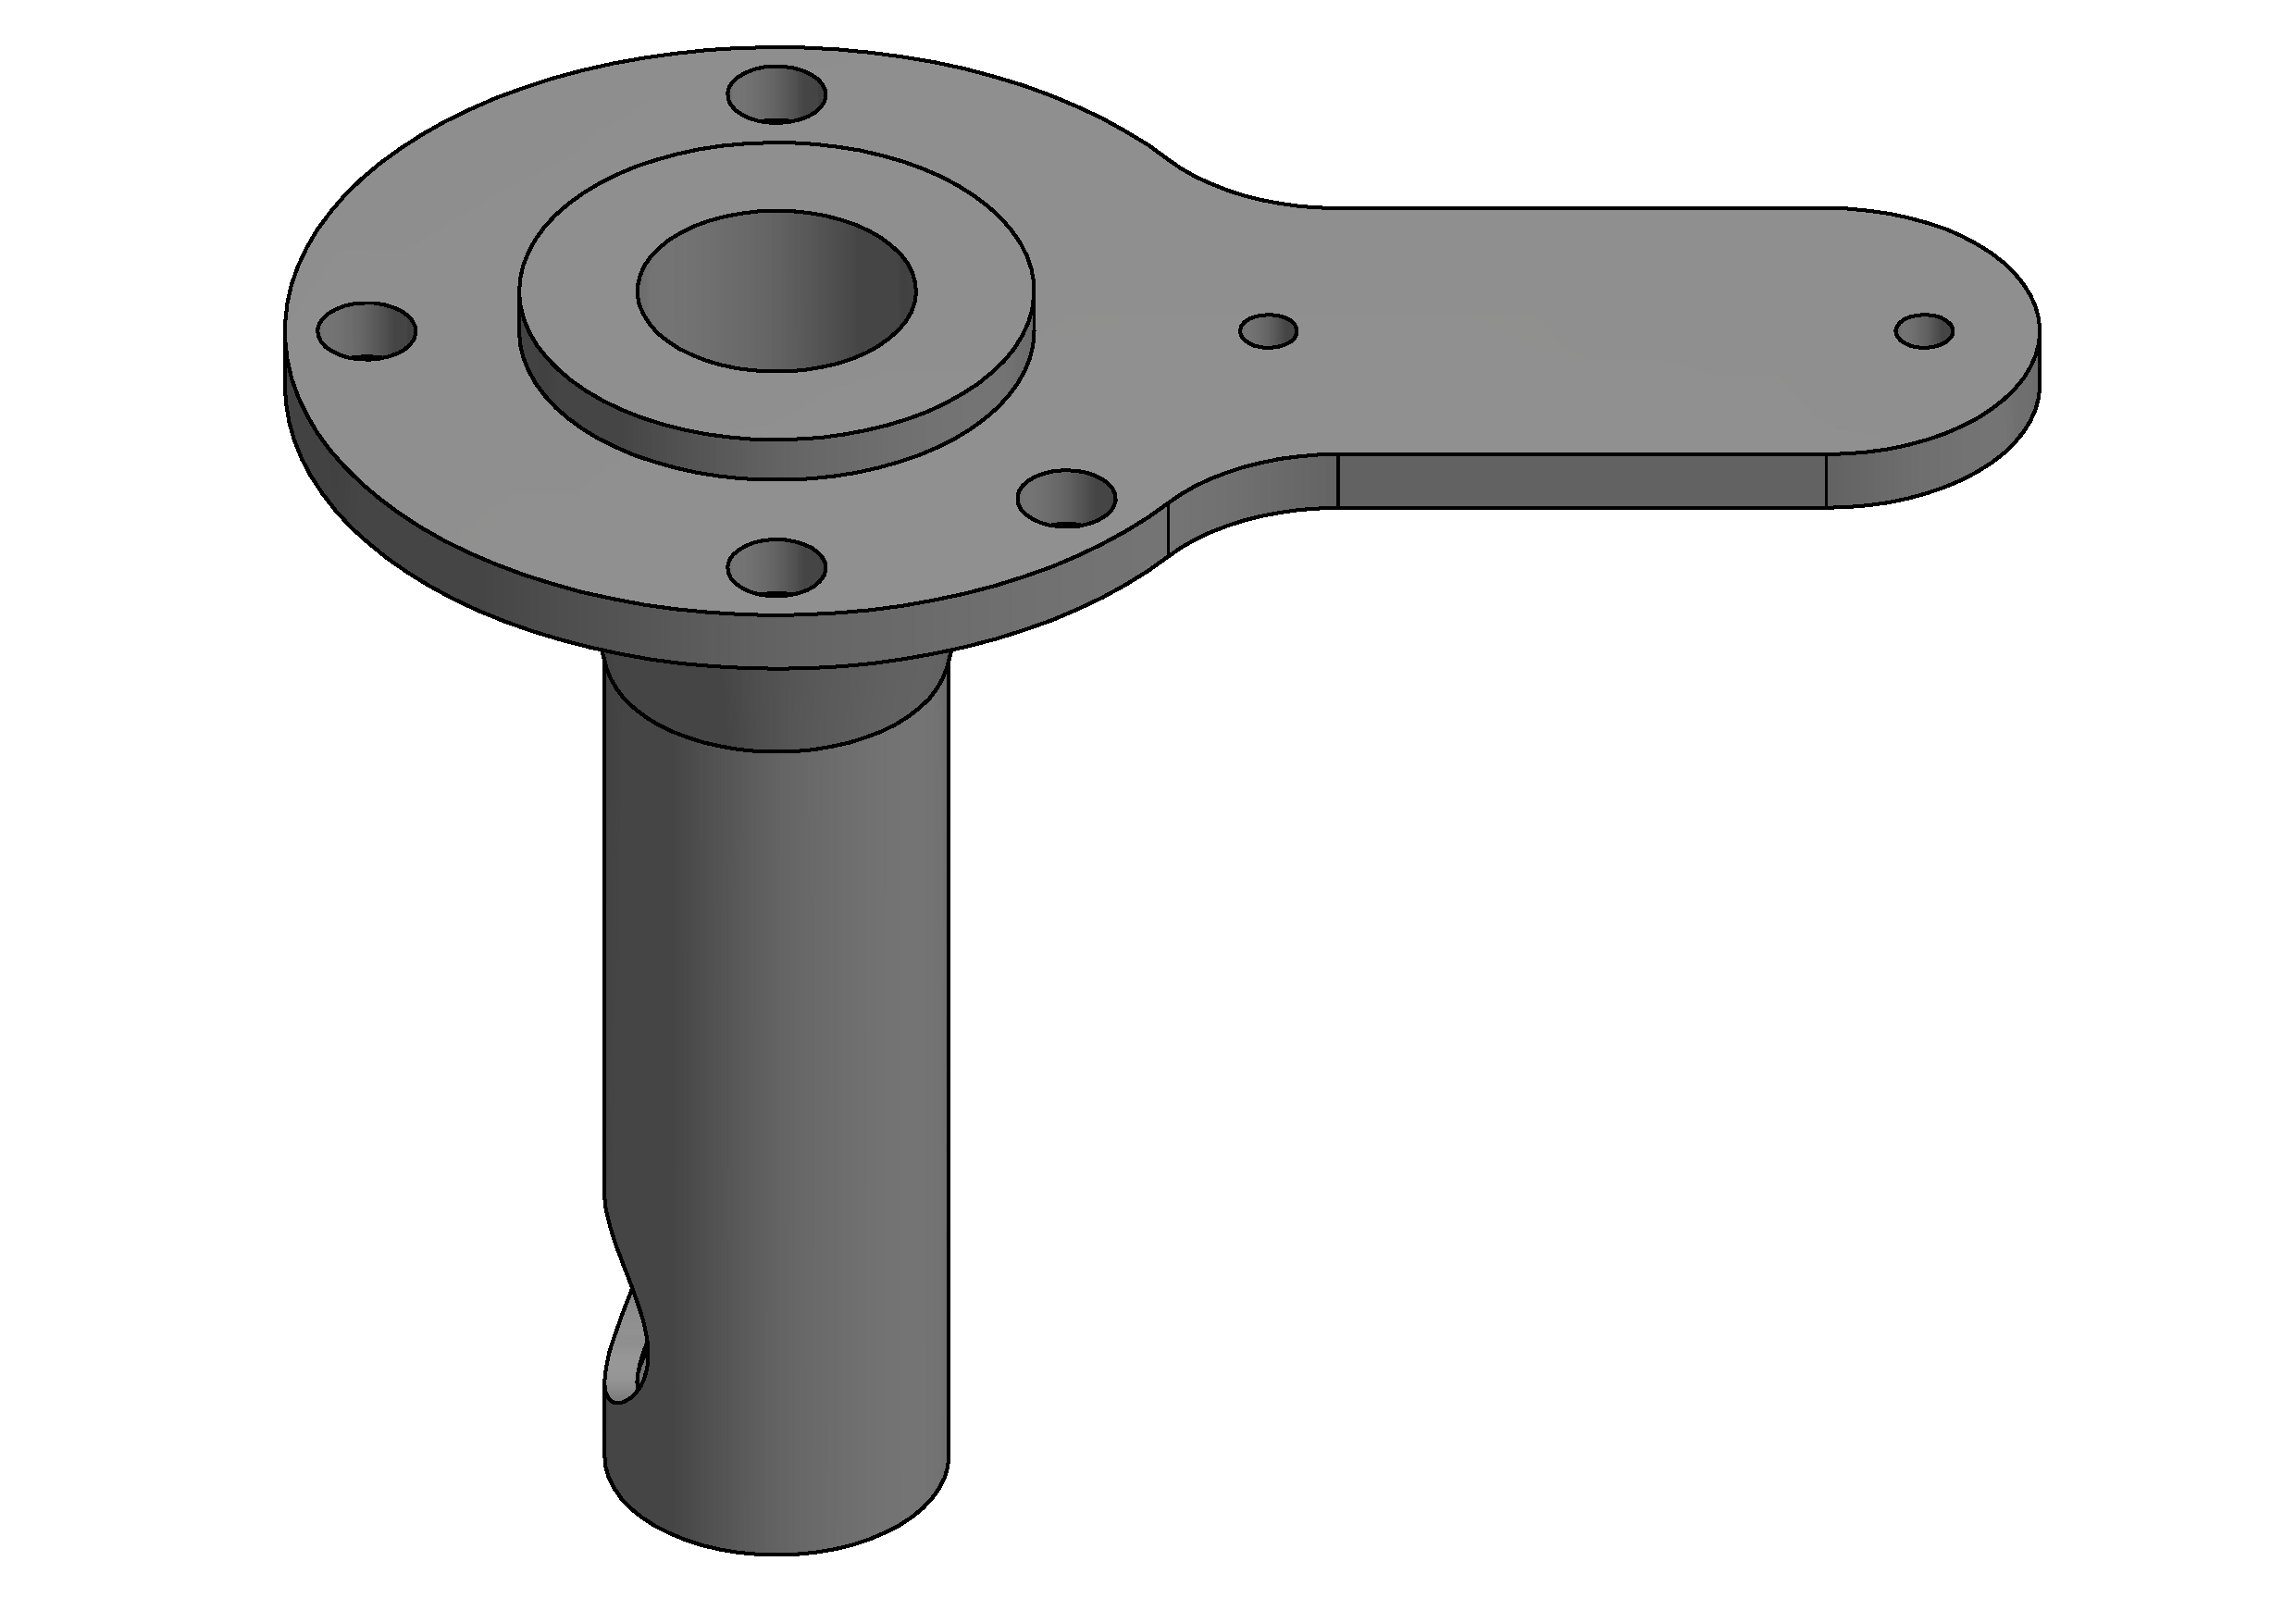
\includegraphics[width=0.48\textwidth]{graphics/single.pdf}}
    \hfill
    \subfloat[Real image of the end effector]{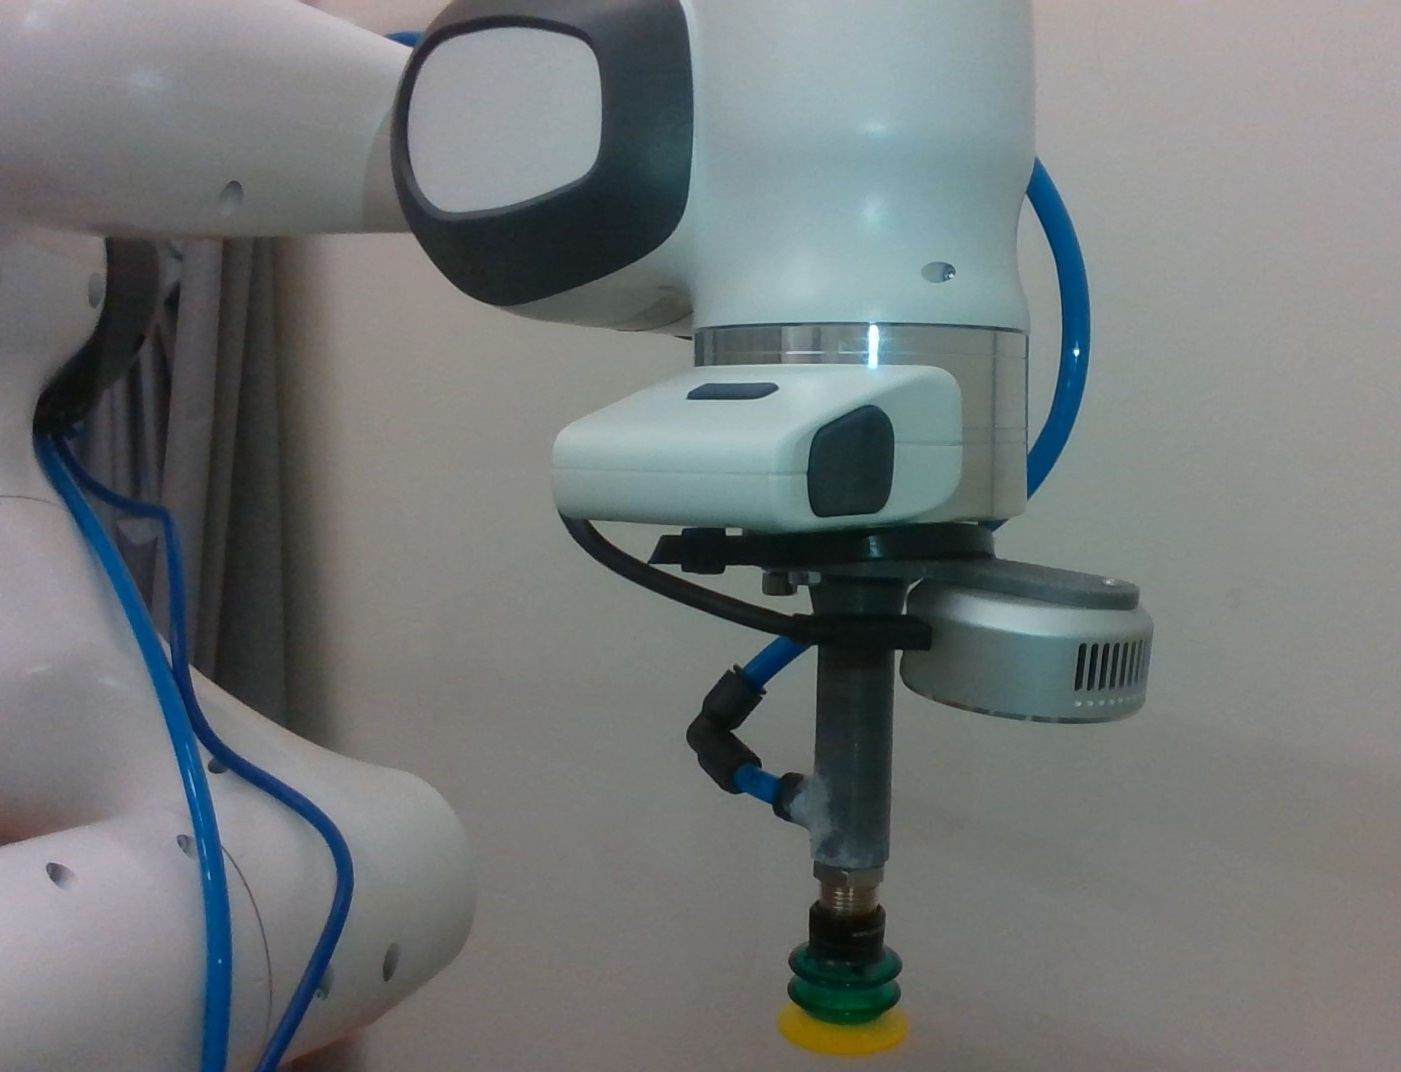
\includegraphics[width=0.48\textwidth]{graphics/endeffector.jpg}}
    %\hfill
    %\subfloat[Real image of the end effector]{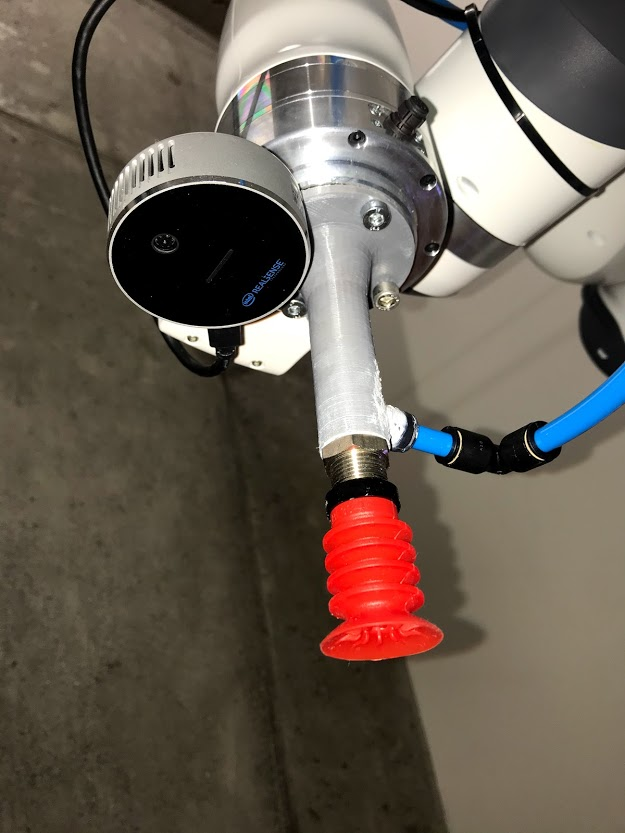
\includegraphics[width=0.25\textwidth]{graphics/rani.jpg}}
    \caption{Robot end effector}
    \label{figure: endeffector}
\end{figure}

\subsection{Camera\label{subsec:camera}} 
In this project, the Intel RealSense LiDAR Camera was used because it generates point clouds with depth information as well as color information from the embedded RGB cameras. The Intel RealSense LiDAR Camera makes use of a proprietary MEMS mirror scanning technology that increases laser power quality. The Intel RealSense LiDAR Camera has a high-resolution FHD RGB camera and an IMU for more reliable handheld scanning. With low power consumption and the ability to produce 23 million precise depth points per second, it's ideal for a wide range of applications. The LiDAR Camera L515 is designed for indoor use with adjustable lighting \cite{noauthor_intel_nodate}.
\begin{figure}[h]
    \centering
    % include first image
    \subfloat[Exploded View]{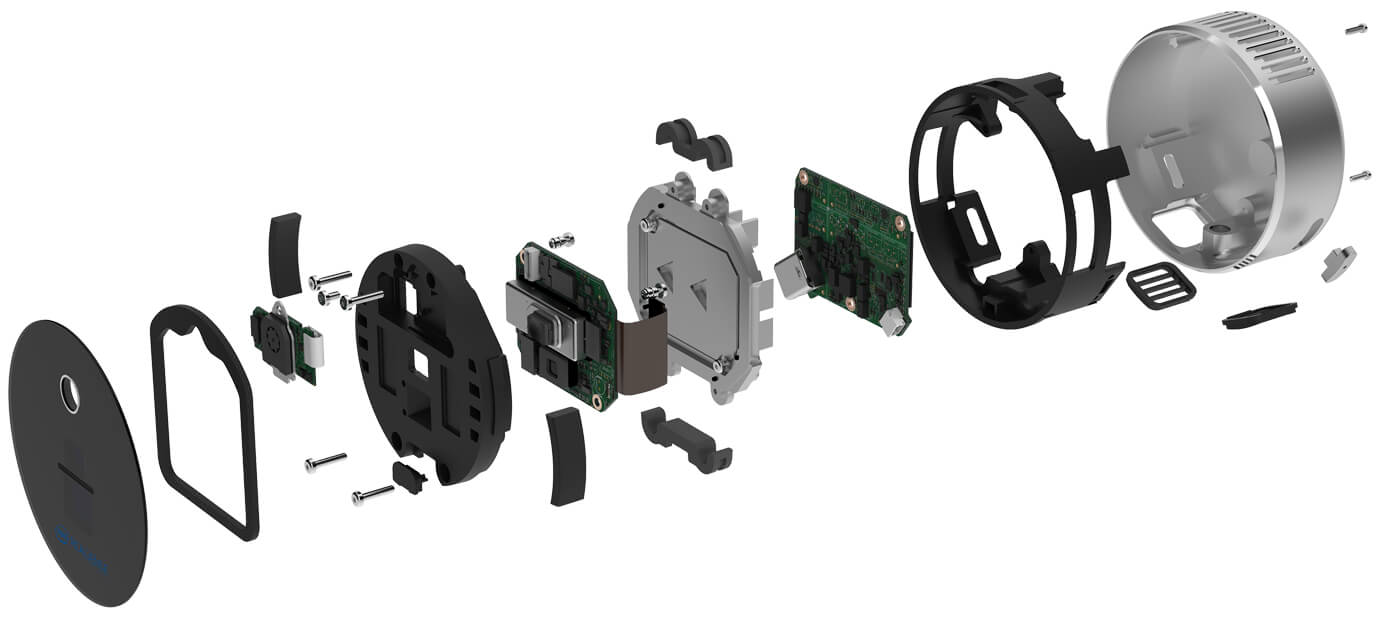
\includegraphics[width=0.6\textwidth]{graphics/Lidar_Camera_L515_detailed.jpg}\label{fig:l515cor}}
    \hfill
    \subfloat[The camera coordinates system]{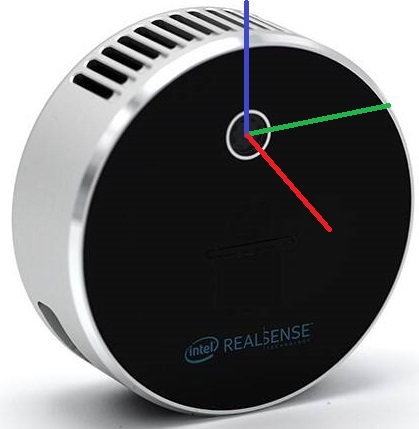
\includegraphics[width=0.30\textwidth]{graphics/lidar515.jpg}}
    \caption{Intel RealSense LiDAR Camera L515 \cite{noauthor_intel_nodate}}
    \label{figure: lidar}
\end{figure}
\clearpage

\section{Code}
Three codes and one launch file were created and used in this project. The panda\_bringup was used to launch the robot, camera, the suction, and the motion planner\textit{(Sec:\ref{sec:pandabringup})}. 
The pick\_and\_place code controls the robot \textit{(Sec:\ref{robotcontrol})}, find\_pickpoint which talks to the camera and uses data to locate items \textit{(Sec:\ref{camera})} and then the difference which finds the difference between before and after picture and labels the images \textit{(Sec:\ref{labelimg})}.

\begin{figure}[h]
    \centering
    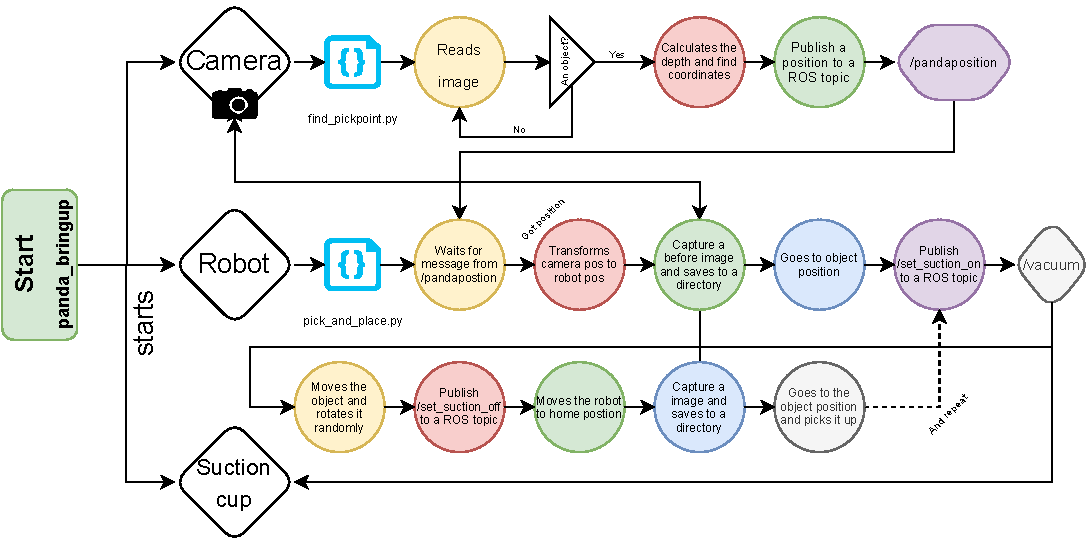
\includegraphics[width=0.9\textwidth]{graphics/softwareDiagram.pdf}
    \caption{Software diagram that shows how the panda\_bringup works}
    \label{fig:softwarediagram}
\end{figure}

A summary of the software diagram, the camera reads images and calculates the depth, the robot picks the object at the desired position and moves it to another position and the suction cup takes commands from the robot.

\subsection{Controlling the robot manipulator}\label{robotcontrol}
The robot manipulator was programmed in python and used ROS to communicate with the robot, the code can be found in the \textit{Appendix \ref{sec:pickandplace}} known as \textit{pick\_and\_place.py}. 
The program starts by creating two ROS publishers, one that talks to the Festo vacuum suction cup and the other that talks to the MoveIt! motion planner. 
It also needs to create a TF(transform) listener so it is possible to read the current positions and orientations, also it can pose transformation between the links. 

When everything has been set up in the program a loop runs while ROS is running. 
Where the robot waits for a message from the find\_pickpoint.py through a ROS topic where it gets an object position from the camera.
The TF listener then transforms the object position in camera coordinates to world coordinates. The robots then move to the object position and pick up the object using the suction cup. When the robot has picked up the object successfully it moves the object to another position and rotates the object. When the robot has successfully moved the object it goes to the home position and takes an image and saves it into a directory. 

\begin{figure}[h]
    \centering
    % include first image
    \subfloat[Starts in home position and capture an image]{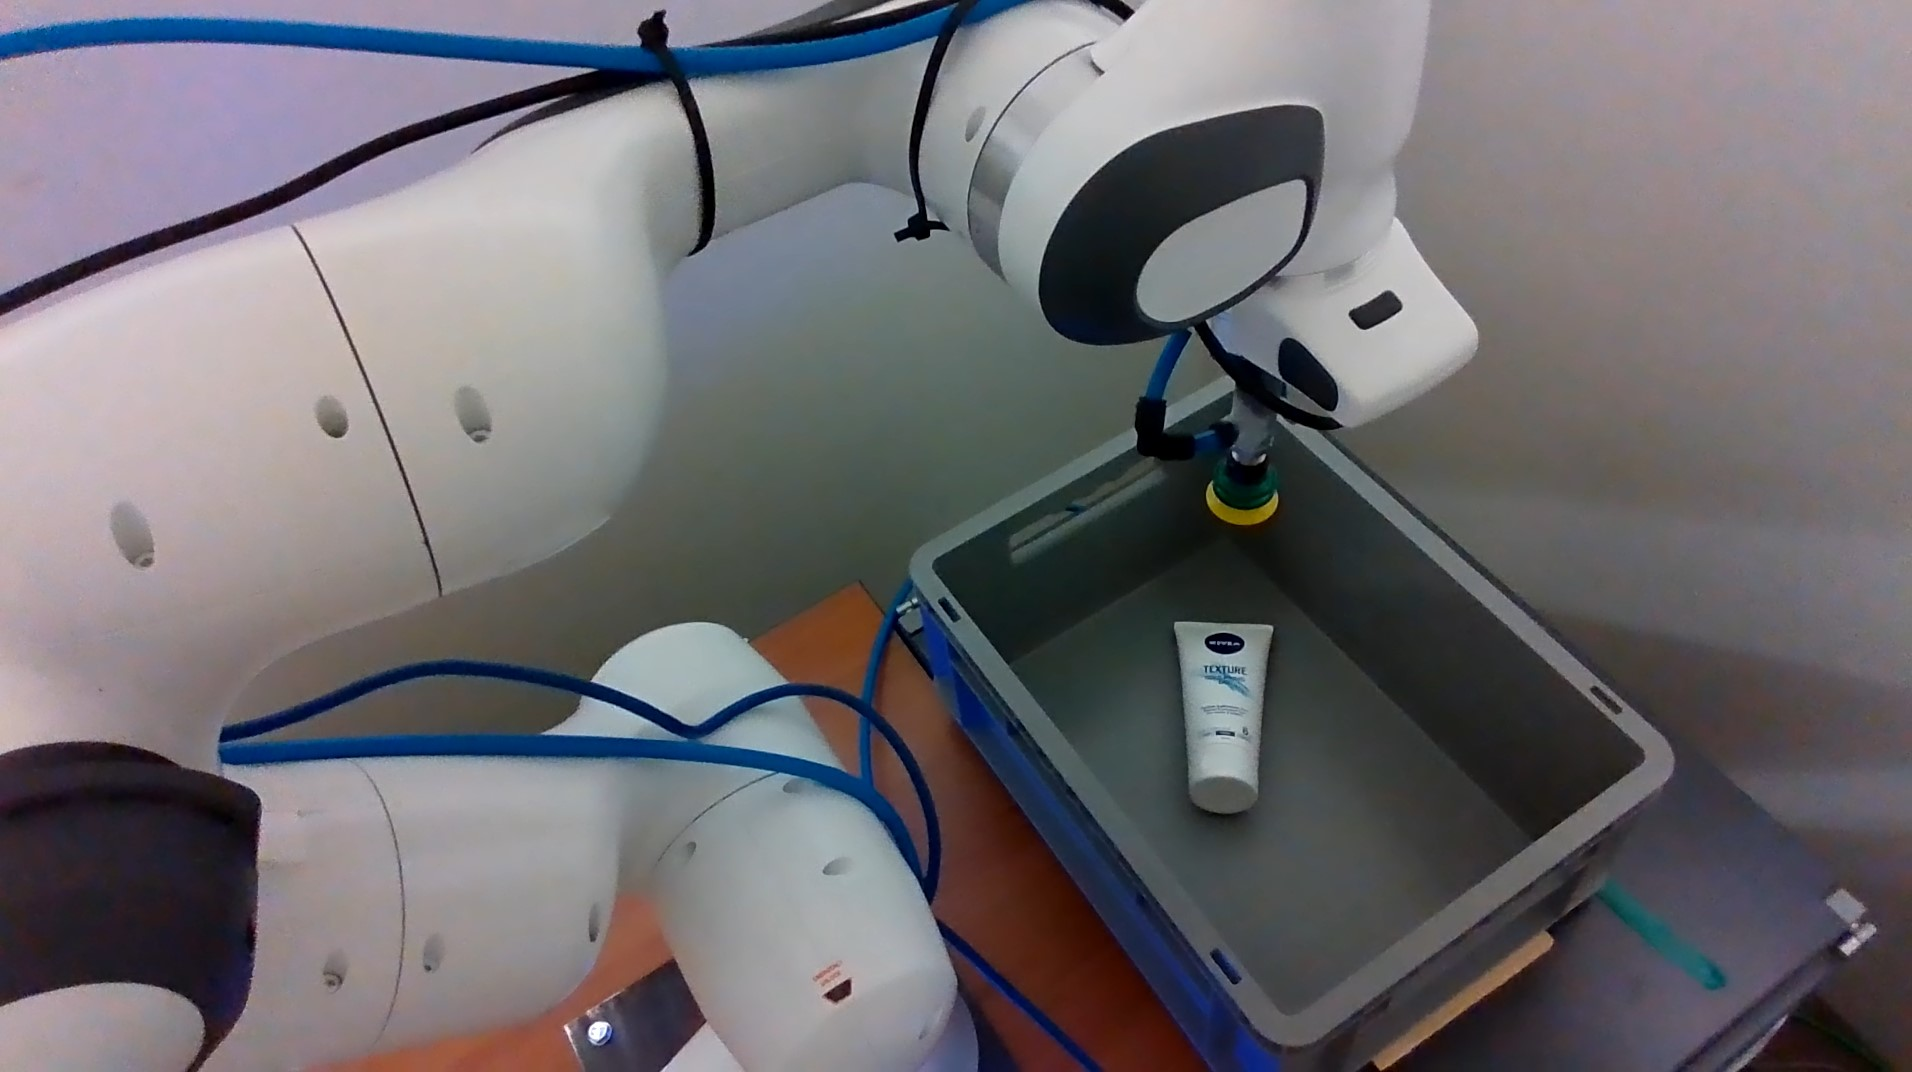
\includegraphics[width=0.33\textwidth]{graphics/results/1home.jpg}}
    \hfill
    \subfloat[Goes to the object]{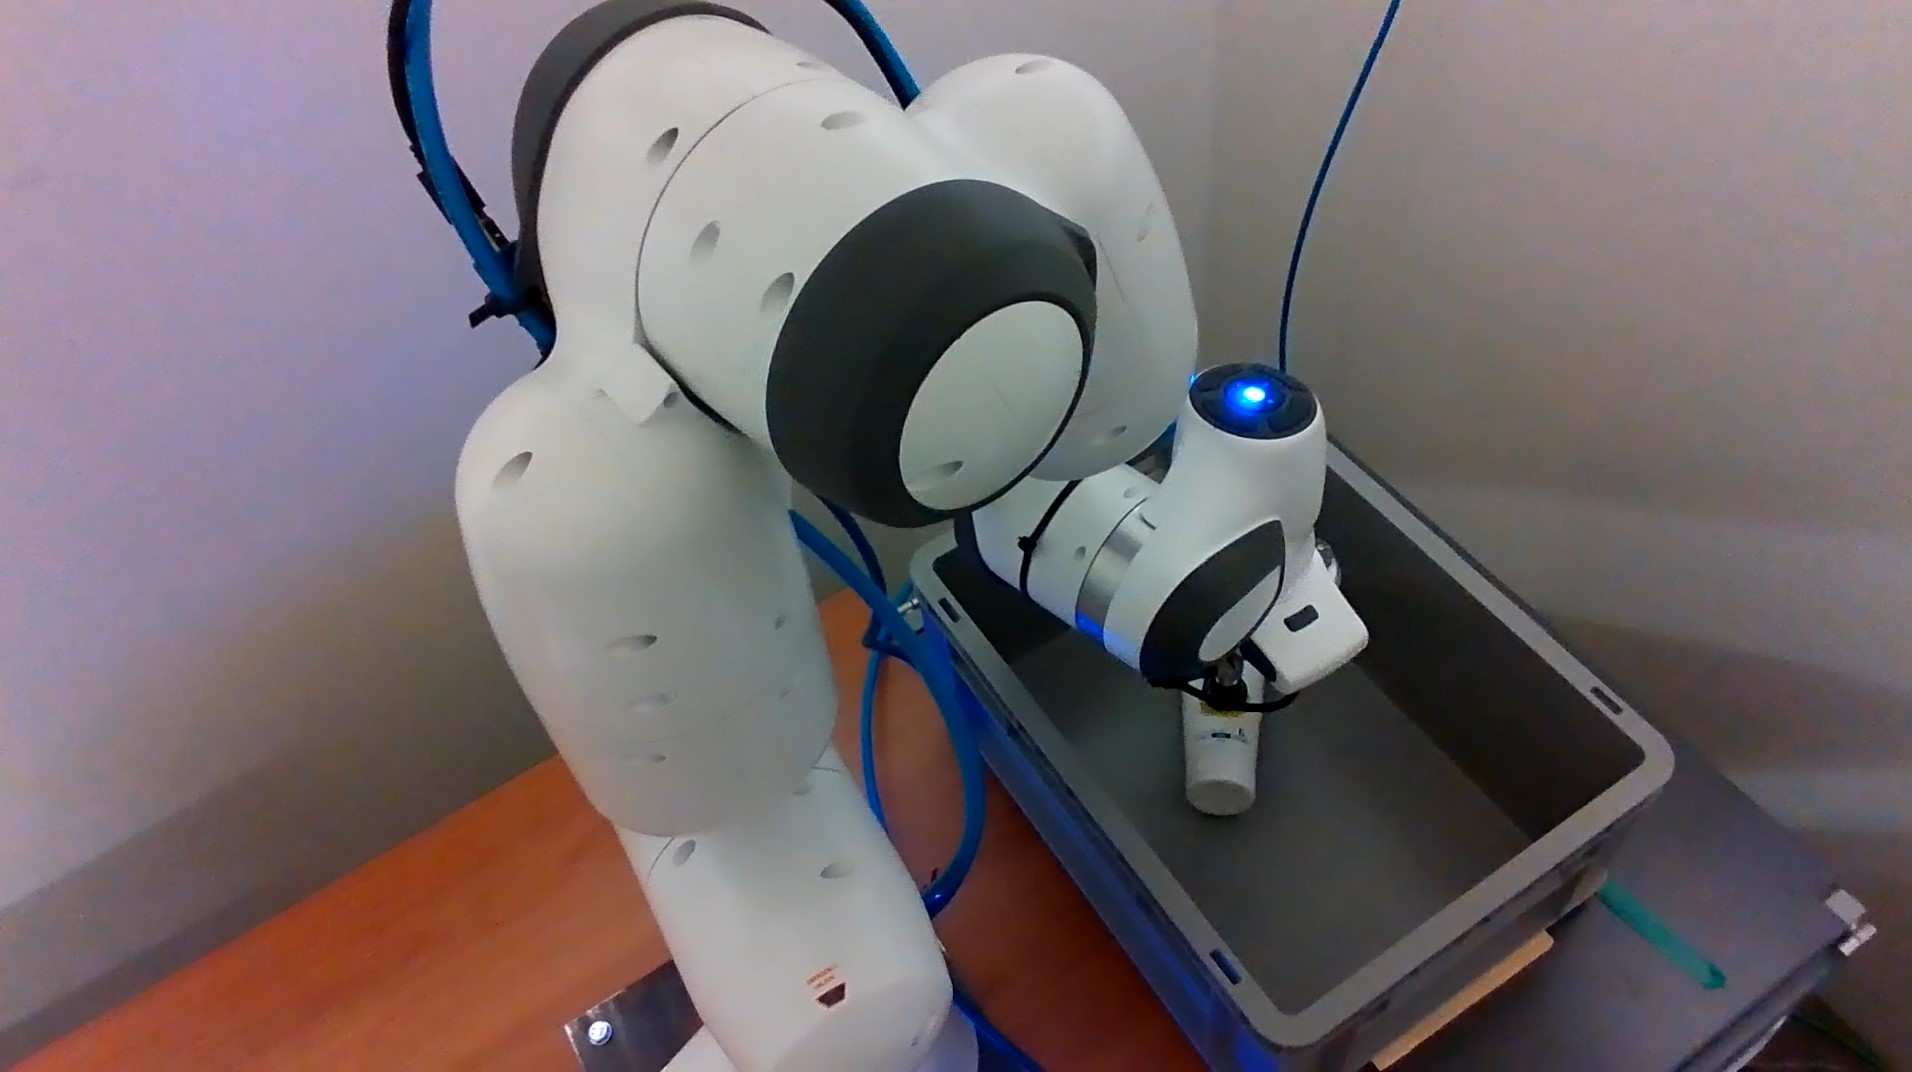
\includegraphics[width=0.33\textwidth]{graphics/results/2pick.jpg}}
    \hfill
    \subfloat[Picks up the object]{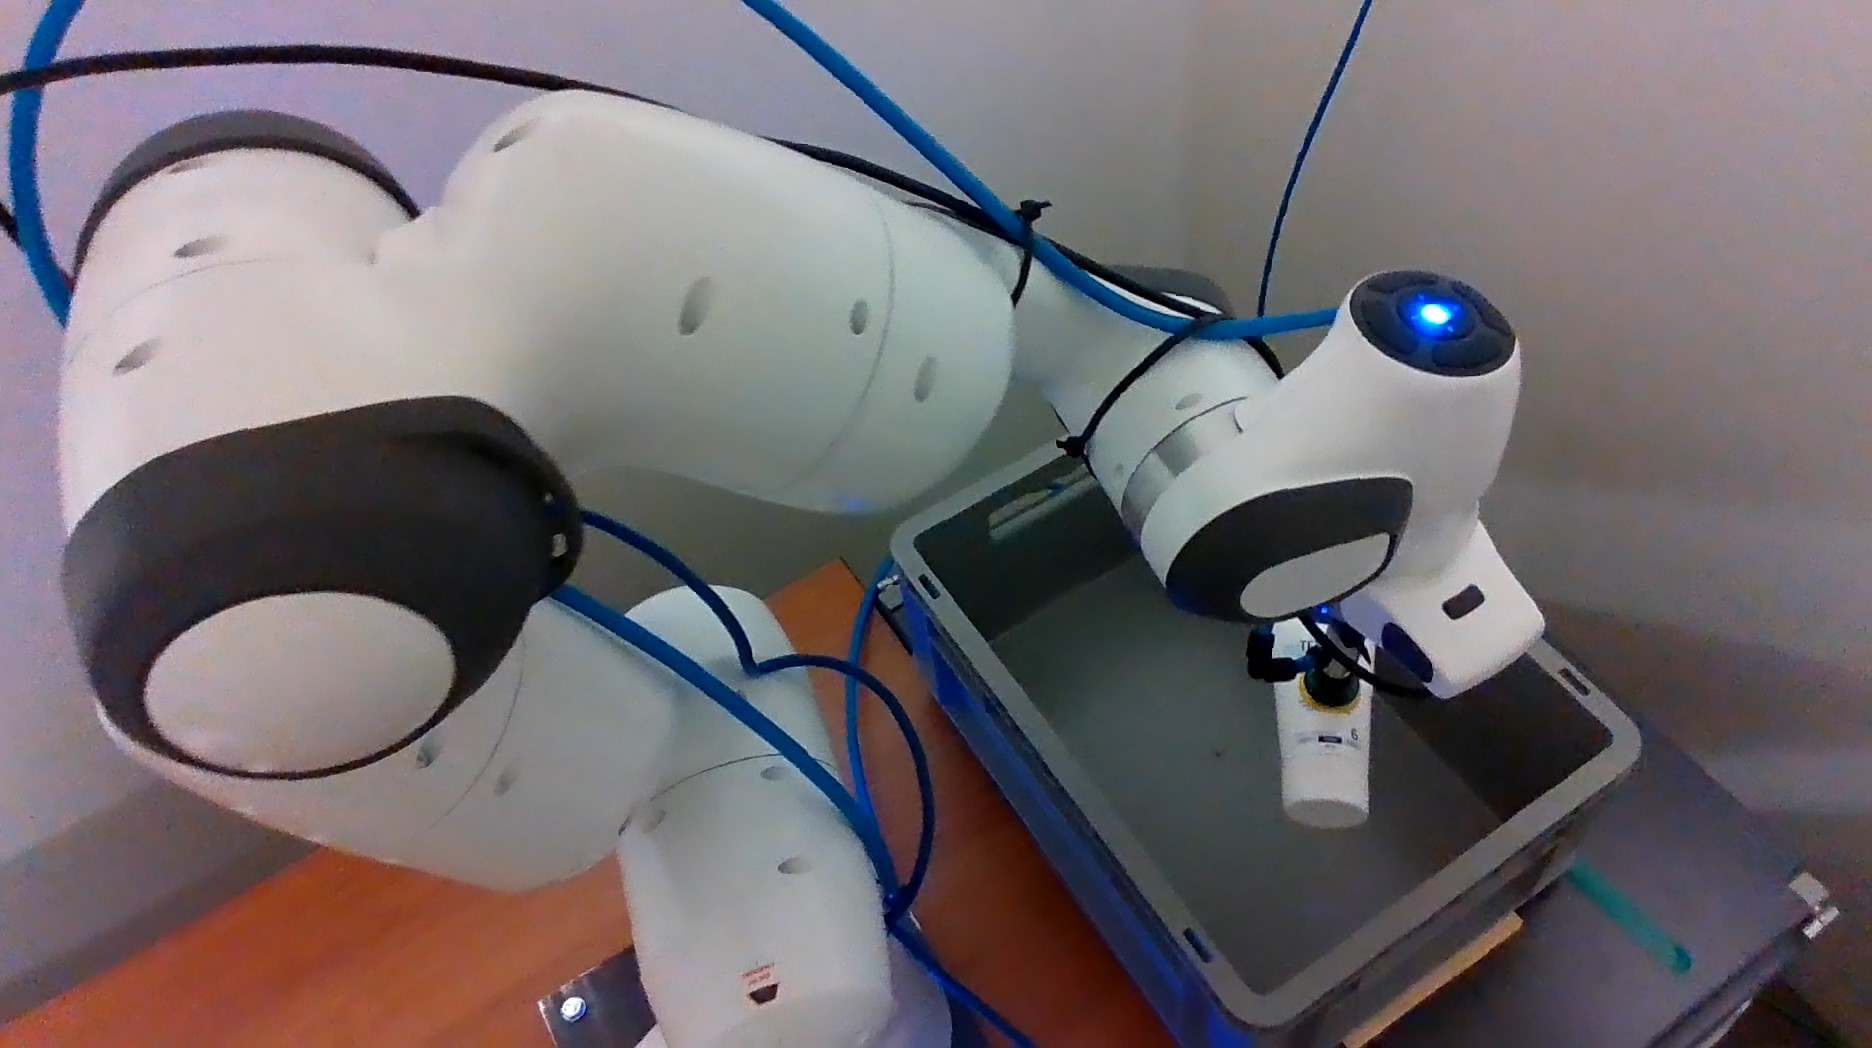
\includegraphics[width=0.33\textwidth]{graphics/results/3move.jpg}}
    \hfill
    \subfloat[Moves the object to another position]{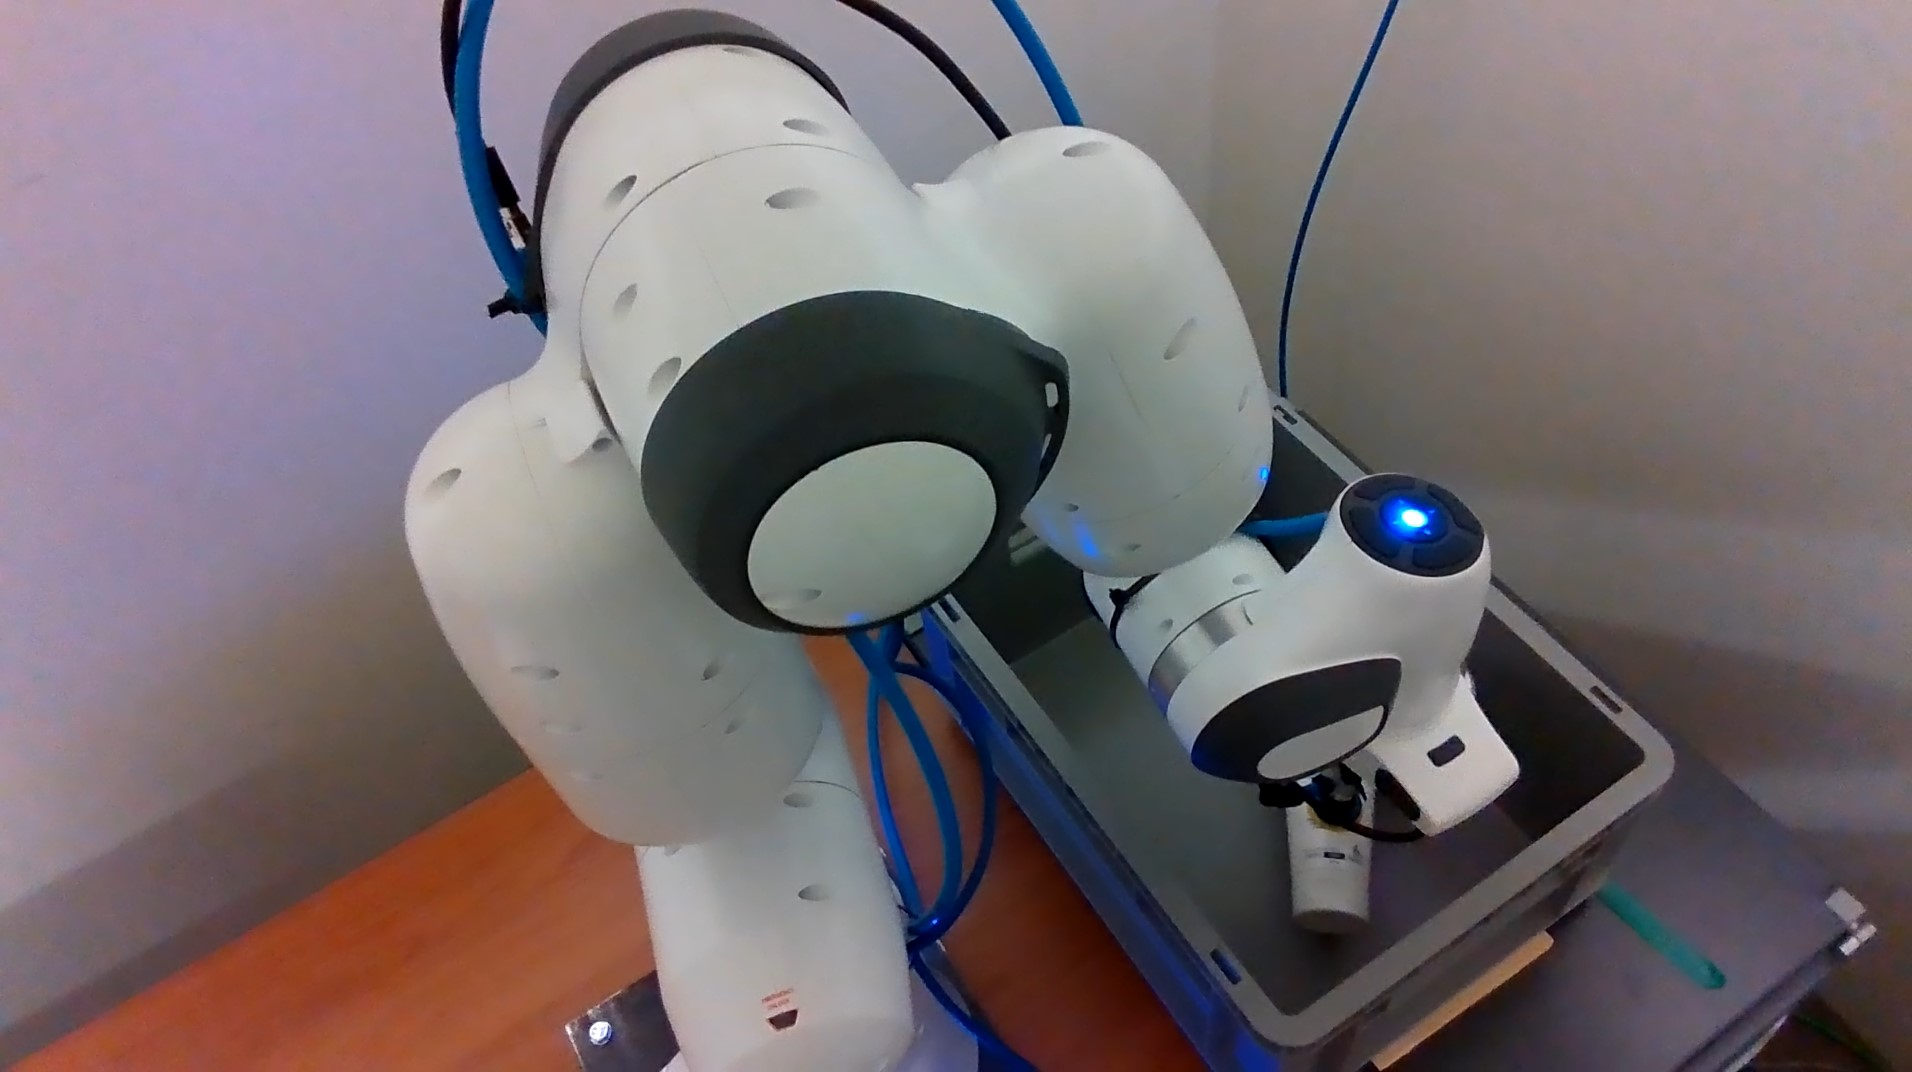
\includegraphics[width=0.33\textwidth]{graphics/results/4above.jpg}}
    \hfill
    \subfloat[Rotates the object and drops it]{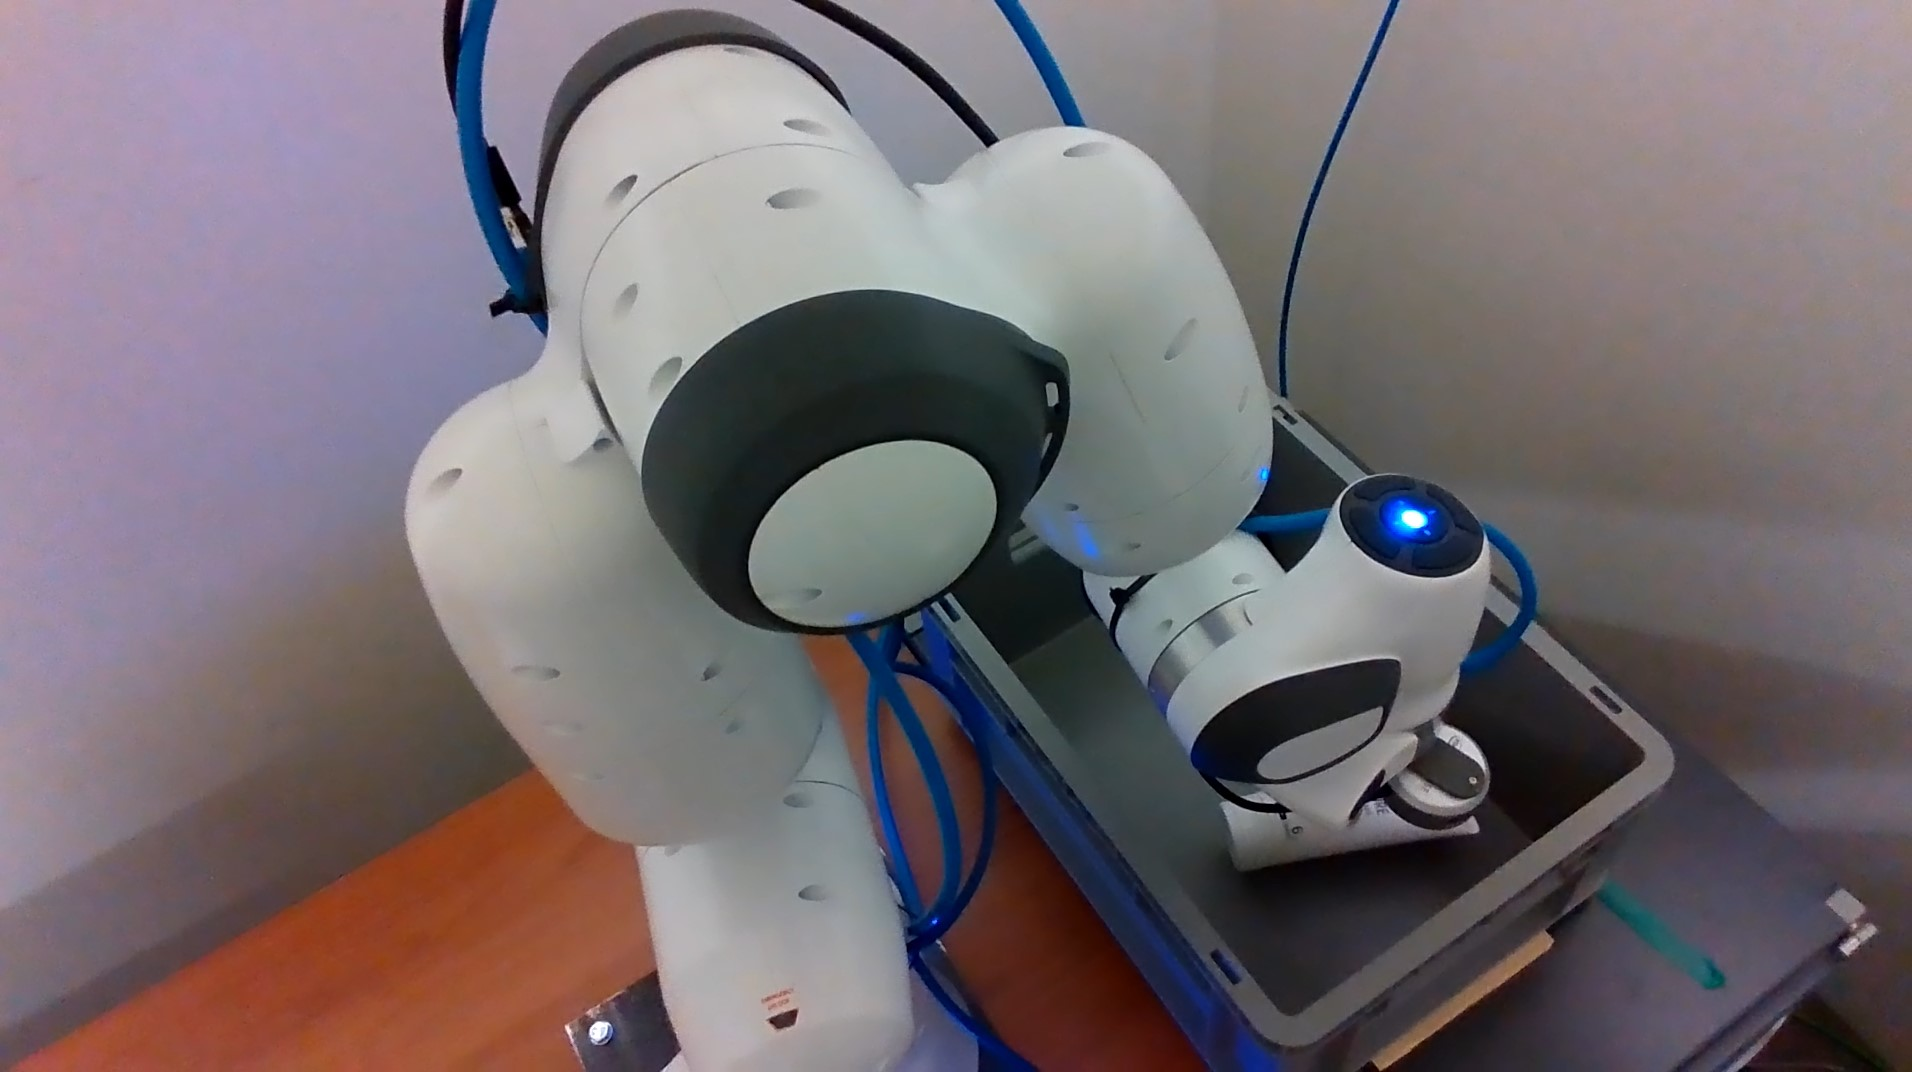
\includegraphics[width=0.33\textwidth]{graphics/results/6rotate.jpg}}
    \hfill
    \subfloat[Goes to home position and capture another image]{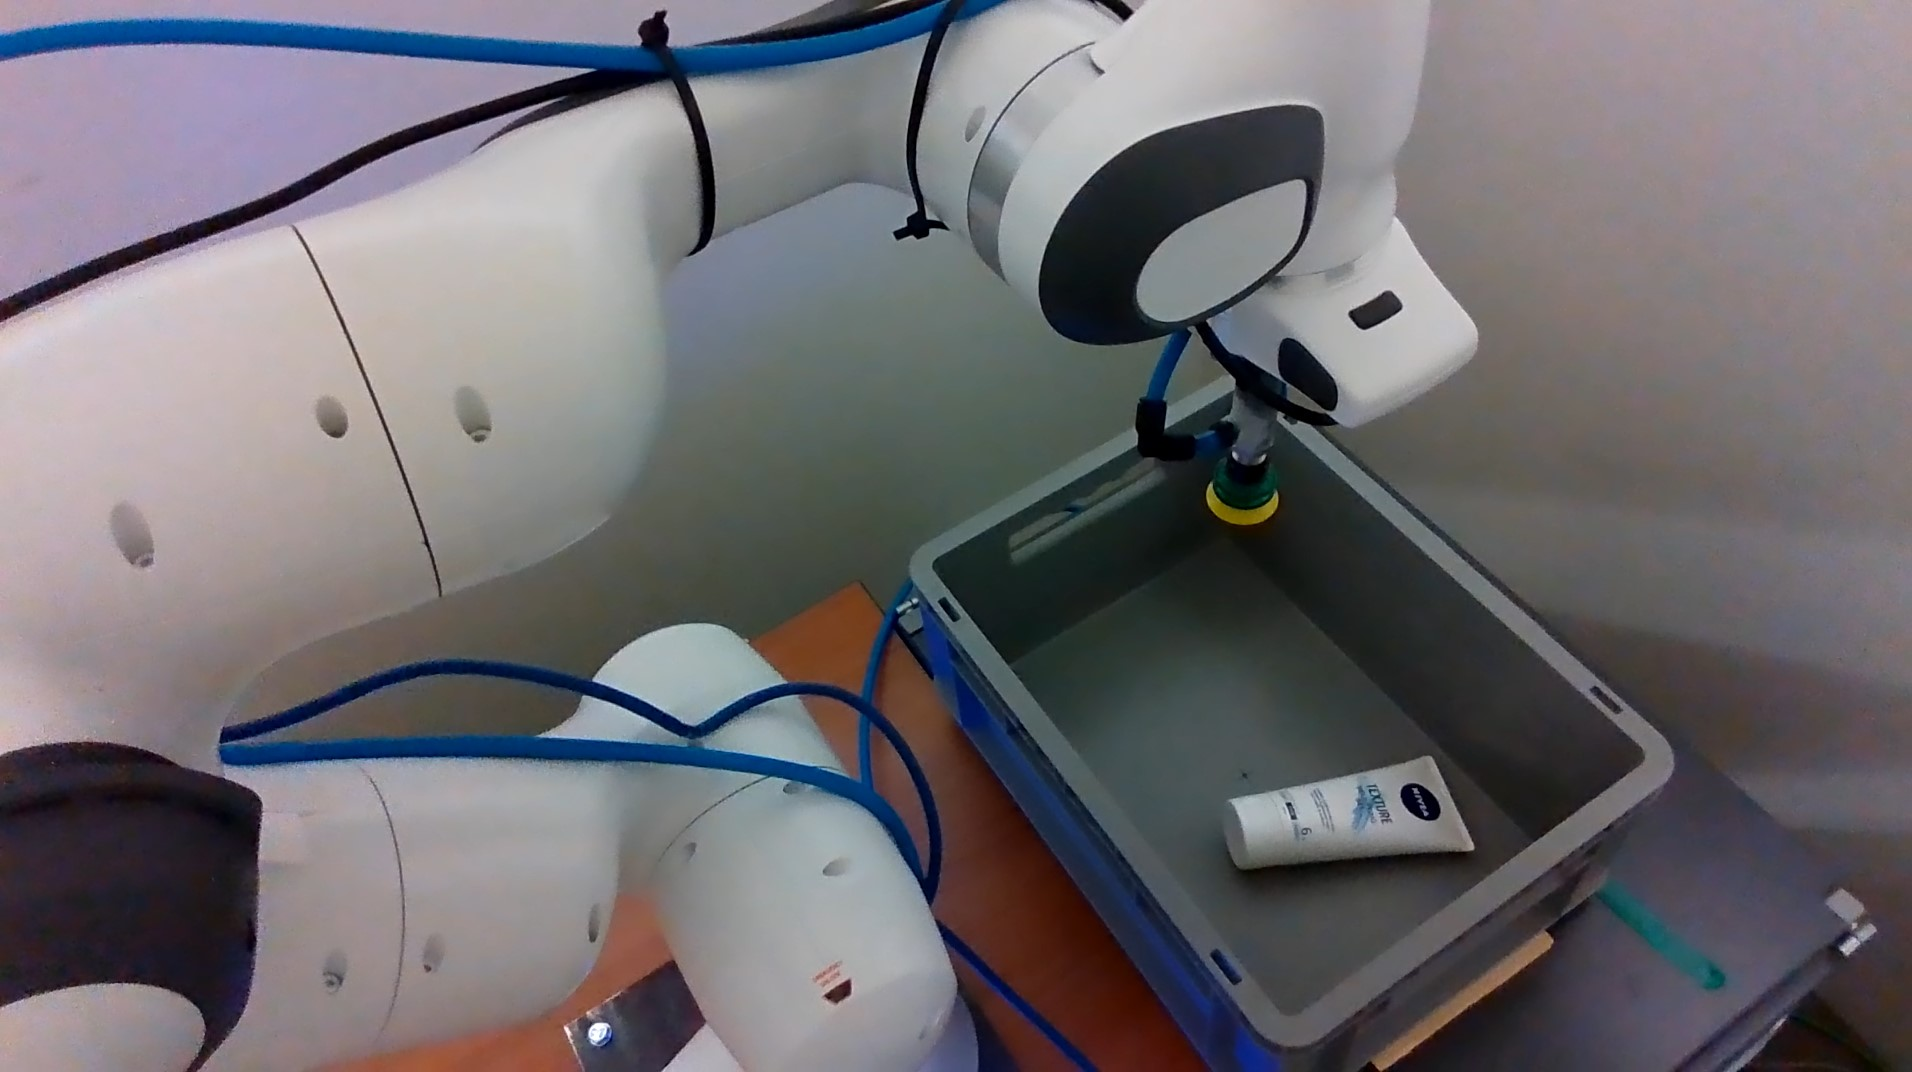
\includegraphics[width=0.33\textwidth]{graphics/results/5drop.jpg}}
    \caption{How the robots works}
    \label{figure: robotworking}
\end{figure}


\subsection{Using the camera}\label{camera}
The camera was used to find the pick point of an object and it was coded in Python and used ROS communication, the code can be found in the \textit{Appendix \ref{sec:findpickpoint}} known as \textit{find\_pickpoint.py}. 
The program starts by initializing a CVBridge class so it can work on images with OpenCV. It then initializes a YOLO neural network and so it can find objects in an image. At last, it creates a subscriber to the "/camera/color/image\_raw" topic with the function "image\_callback" as a callback and creates a publisher "pandaposition" that talks to the robot manipulator. Then a loop keeps the program from shutting down unless ROS is shut down.

When the callback gets an image it waits for an aligned depth to a color image so it can read a depth at a certain point. It then goes into a find objects function that finds the object in the image using the neural network, which locates the center of an object. When the program has found pixel coordinates of the object it can find the depth at that point and can create real-world coordinates(X, Y, Z) in meters at the camera location. At last, the programs send the real-world coordinates to a "pandaposition" publisher so the robot manipulator uses the coordinates.

\begin{figure}[h]
    \centering
    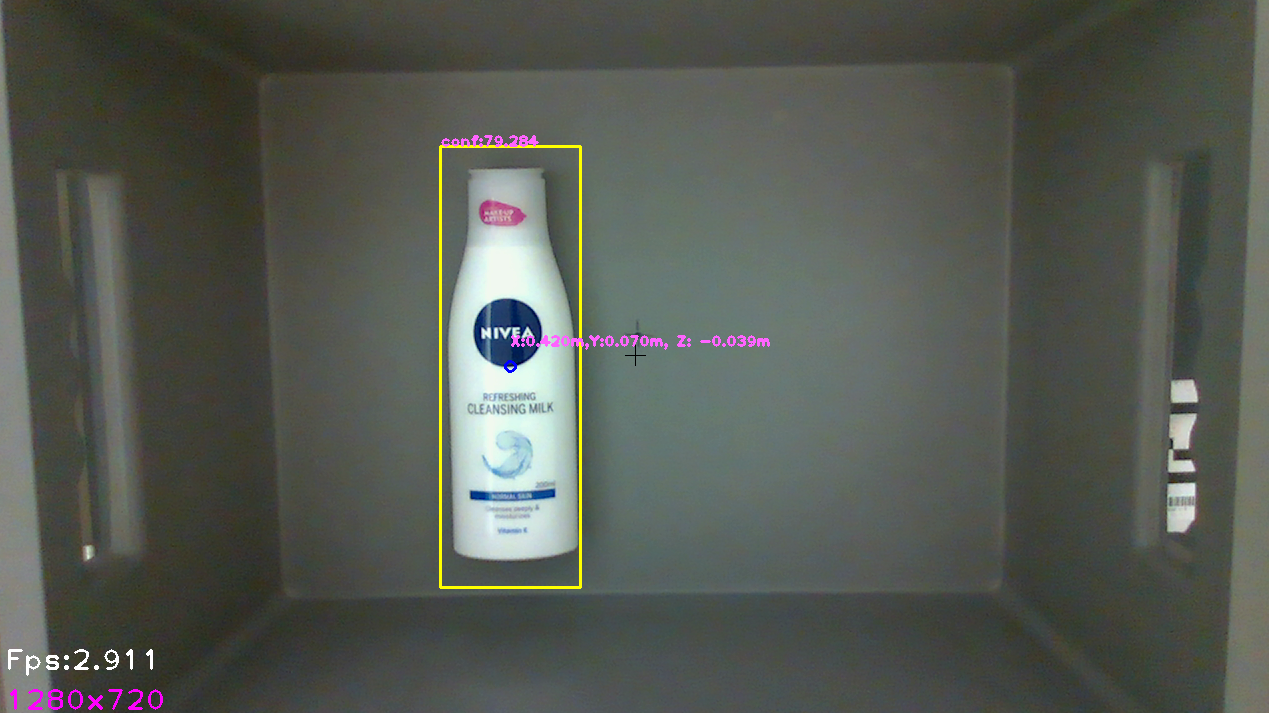
\includegraphics[width=0.8\textwidth]{graphics/findpickpoint.png}
    \caption{An example of the output from the find\_pickpoint.py code}
    \label{fig:findpickpoint}
\end{figure}

From \textit{Figure \ref{fig:findpickpoint}} you can see the confidence, frames per second(Fps), image size, X which is forward length or depth, Y and Z is the distance from the center of the camera in meters. 
The camera coordinates system can been seen in \textit{Figure \ref{fig:l515cor}}.


\subsection{Labelling the images}\label{labelimg}
When the robot manipulator and camera had collected images, the images were put in a program called \textit{difference.py} and can be found in the \textit{Appendix \ref{sec:difference}}. That program was coded in Python and works individually. The program locates objects in the images and labels them. 
\subsubsection*{Before vs. After}\label{beforeandafter}
The first method used before- and after- image, the bottle was moved to the other side and then found the difference. It calculates the Structural Similarity Index (SSIM) between the two images and then used the OpenCV threshold and contours to draw the contours. Then iterate around the contour area, and get a bounding area and draw a rectangle around.
An example of input images can been seen in \textit{Figure \ref{figure: beforeafter}}, and try's to find the difference between before and after.
\begin{figure}[h]
    \centering
    % include first image
    \subfloat[Before]{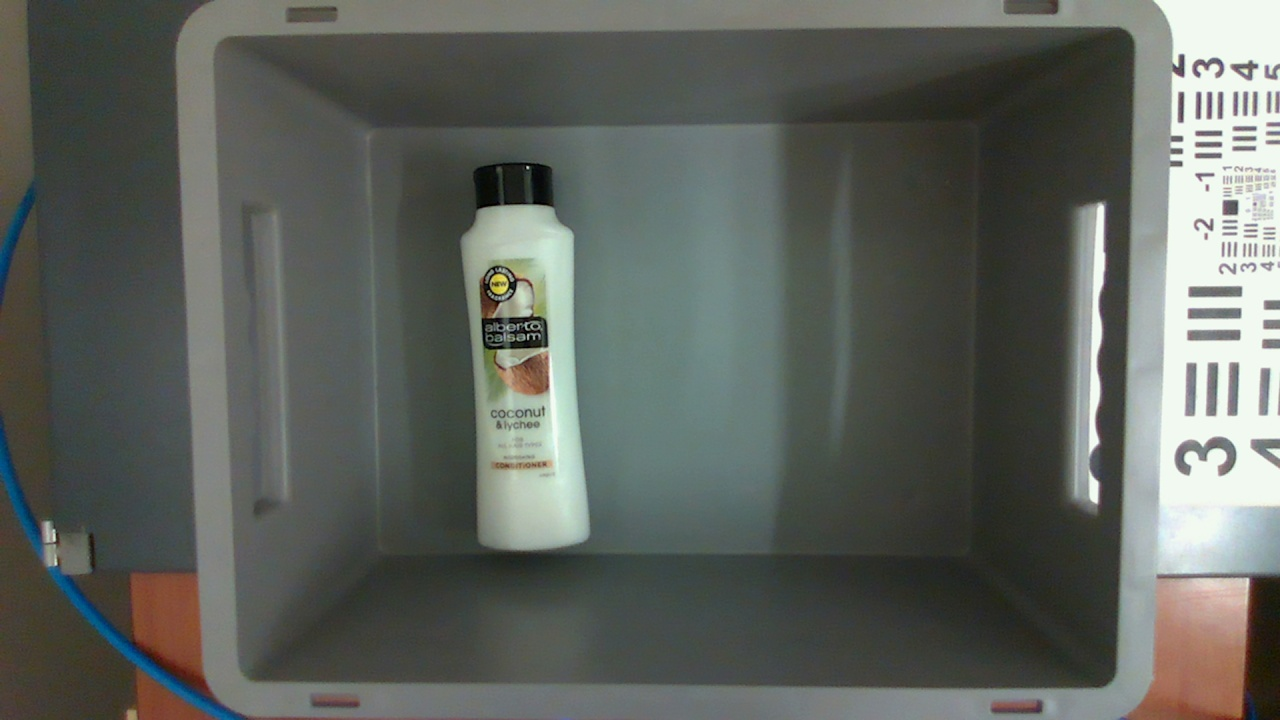
\includegraphics[width=0.45\textwidth]{graphics/methods/frame0000.jpg}}
    \hfill
    \subfloat[After]{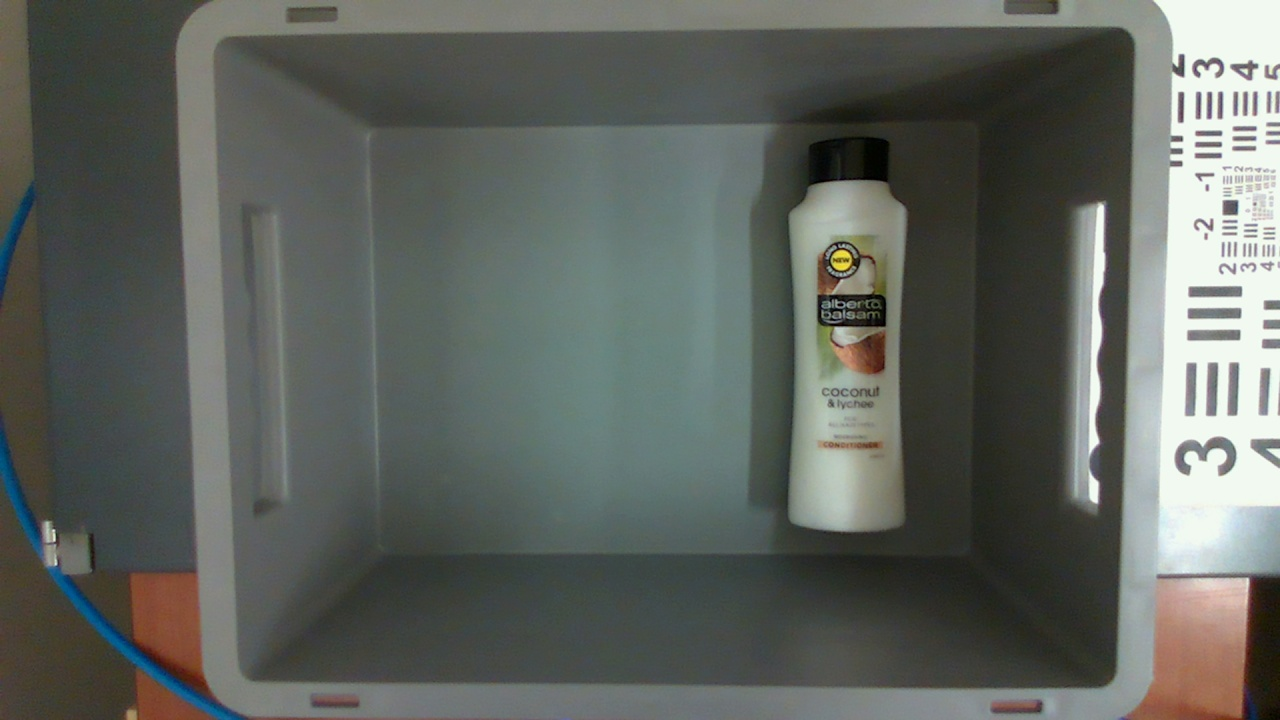
\includegraphics[width=0.45\textwidth]{graphics/methods/frame0001.jpg}}
    \caption{An example of input images}
    \label{figure: beforeafter}
\end{figure}

\subsubsection*{Empty bin vs. item in the bin}\label{emptyvsitem}
The second method uses two functions to find objects in the image, one is to find the difference between an empty bin and a bin with an object inside and the other is to find contours in the image. 
The function that delivers better results is used or if the results are similar average values are used. 
In this program, OpenCV and Skicit-image are used. 
So the program starts by getting an image of an empty bin and then the images with an object in it. 
Then it finds uses \textit{cv2.Canny} to find the edges, creates a binary threshold image with \textit{cv2.threshold} and finds the contours from the threshold image.  
When the contours have been found it goes to a function that checks if the contour has four corners to check if it is a rectangle. 
If it has four corners and the area is within area marks it saves the location\textit{(center point, width, and height relative to the image size)} of the object in a text file named the same as the image. 
When the program has finished with the all images an text file with locations of objects for each image, is saved and can be used to train the neural network. An example of input images can been seen in \textit{Figure \ref{figure: emptyafter}}.
\begin{figure}[h]
    \centering
    % include first image
    \subfloat[Empty bin]{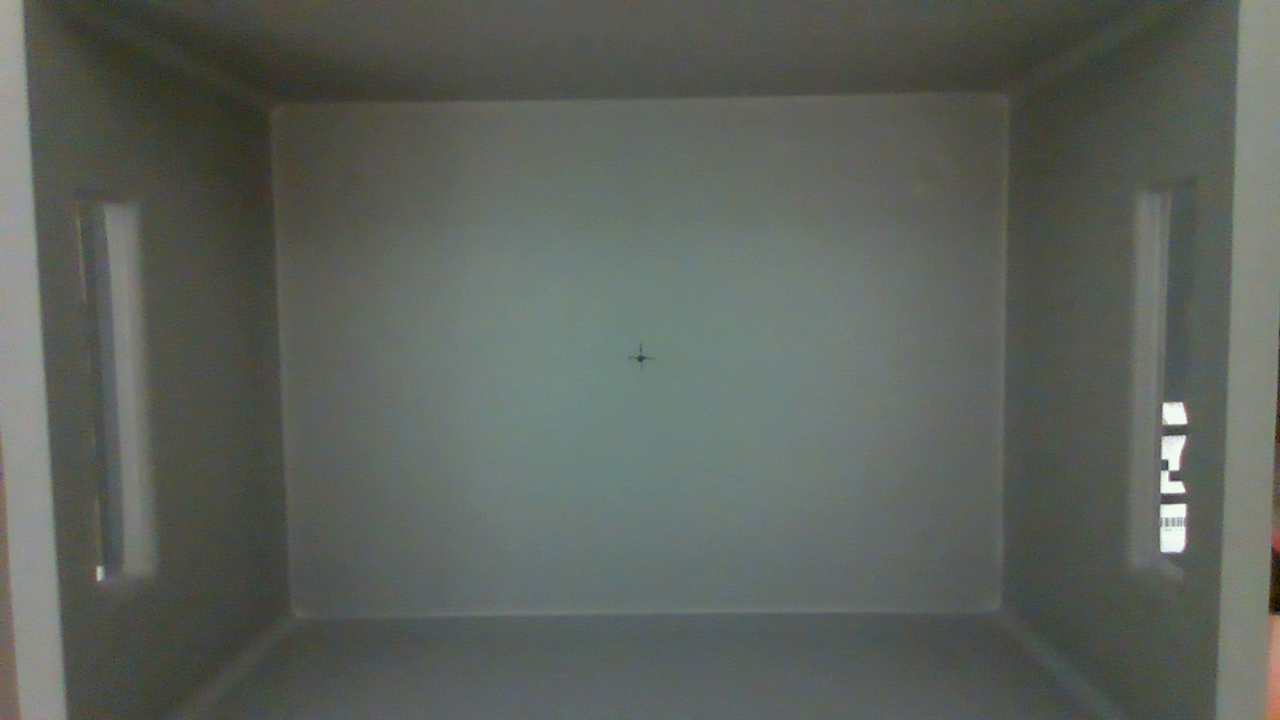
\includegraphics[width=0.45\textwidth]{graphics/methods/0000.png}}
    \hfill
    \subfloat[Item in the bin]{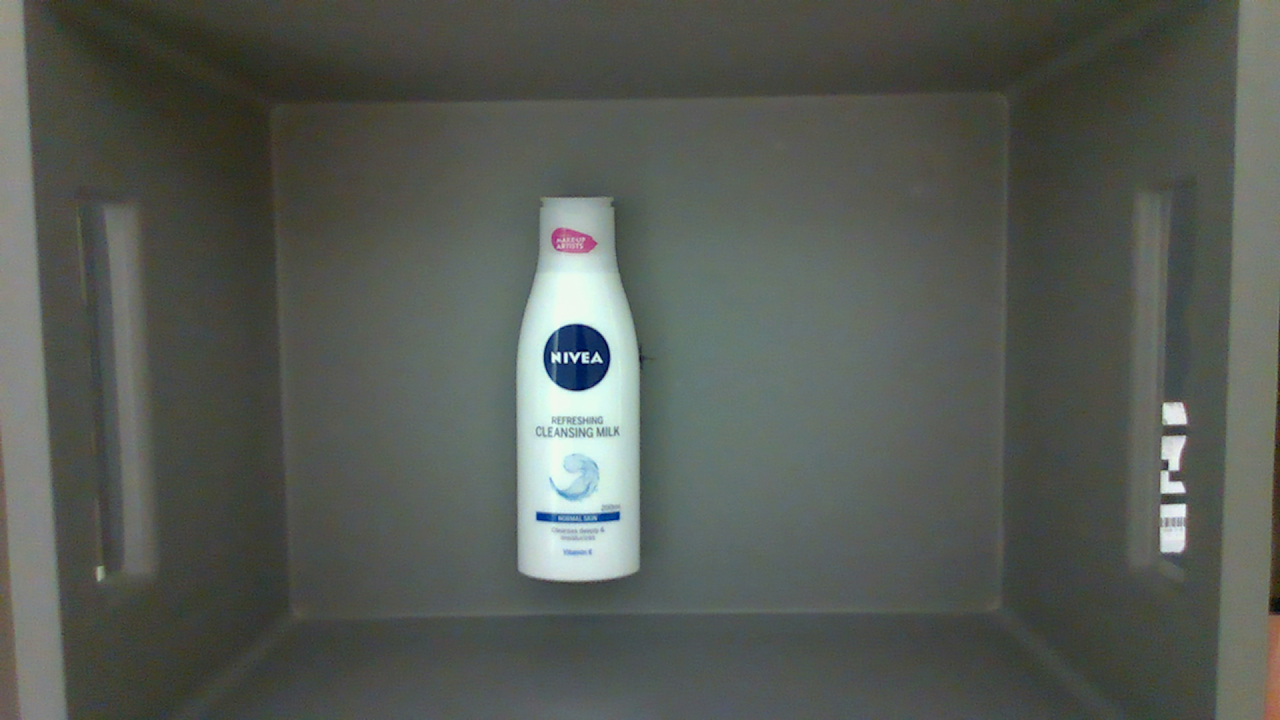
\includegraphics[width=0.45\textwidth]{graphics/methods/0001.png}}
    \caption{An example of input images}
    \label{figure: emptyafter}
\end{figure}
\clearpage
\section{Beiersdorf dataset}
A Beiersdorf dataset\cite{bjarnason_1984-_detecting_2021} was used in this project as a test dataset, it was created by a former master's student in Reykjavík University. 
The dataset consists of 15 products. The data set included 145 images per item, up to 2,175 of which were taken. This dataset is diverse, with similar items and also items that have different shapes. It should therefore provide a good indication for future work. \textit{Figure \ref{fig:beiersdorf}} below shows the items that are in the dataset.

% \begin{figure}[h]
%     \centering
%     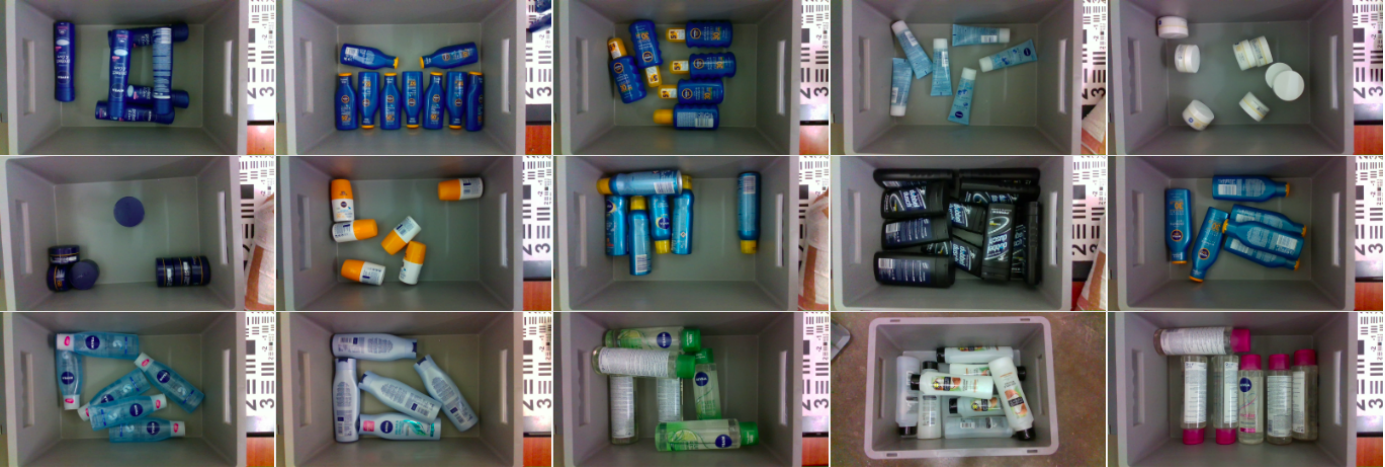
\includegraphics[width=1\textwidth]{graphics/methods/sverrirdataset.PNG}
%     \caption{Beiersdorf dataset contains 15 items\cite{bjarnason_1984-_detecting_2021}}
%     \label{fig:beiersdorf}
% \end{figure}

\begin{figure}[h]
    \centering
    % include first image
    \subfloat[Item 1]{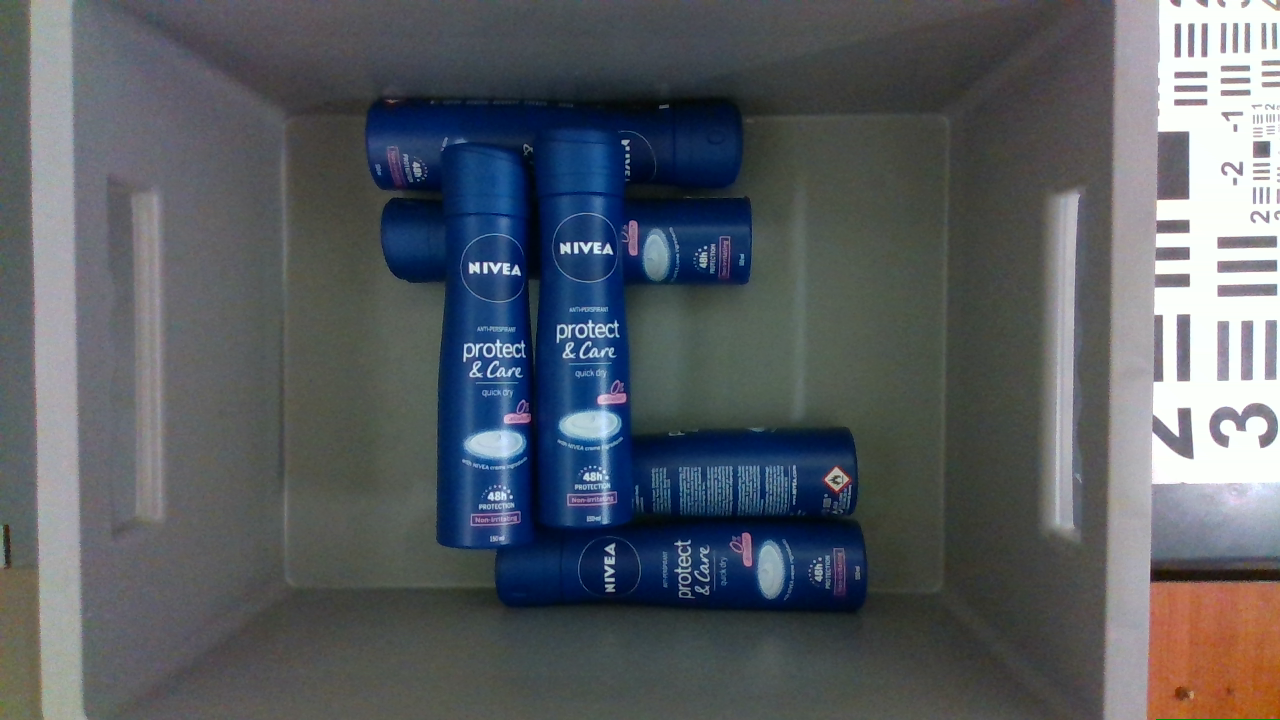
\includegraphics[width=0.2\textwidth]{graphics/beiersdorf/i0001.png}}
    \hfill
    \subfloat[Item 2]{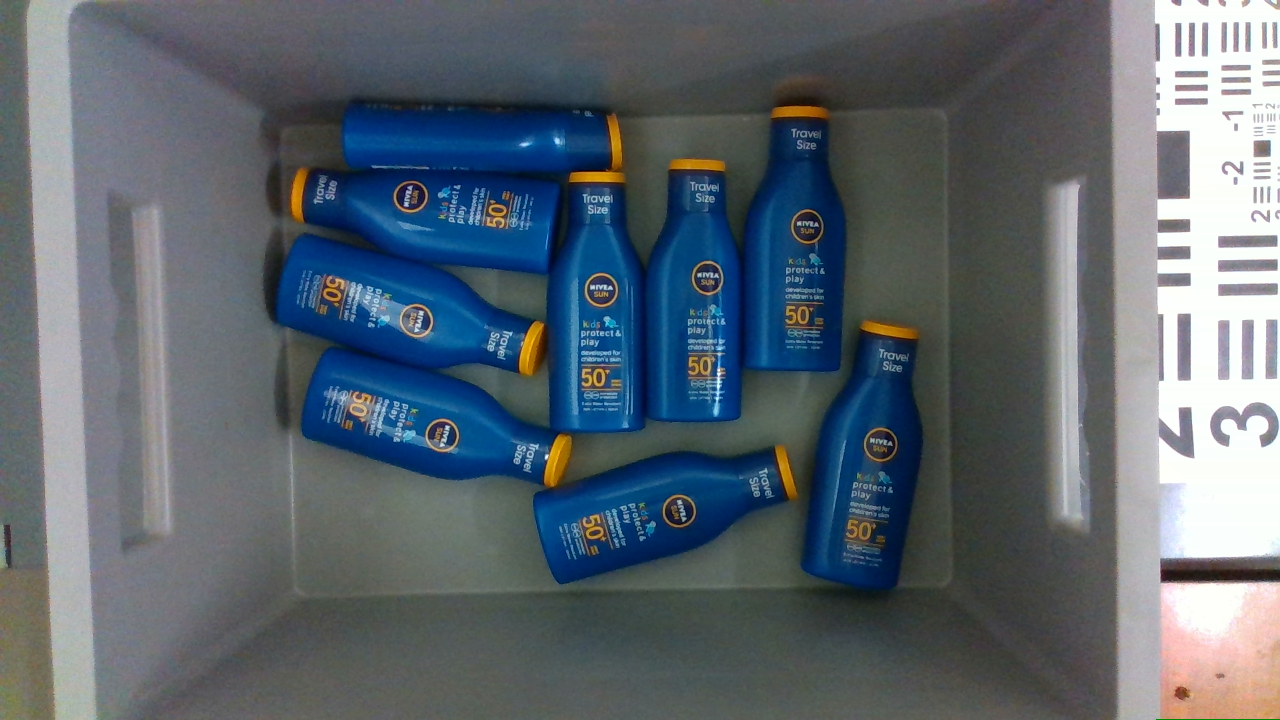
\includegraphics[width=0.2\textwidth]{graphics/beiersdorf/0155.png}}
    \hfill
    \subfloat[Item 3]{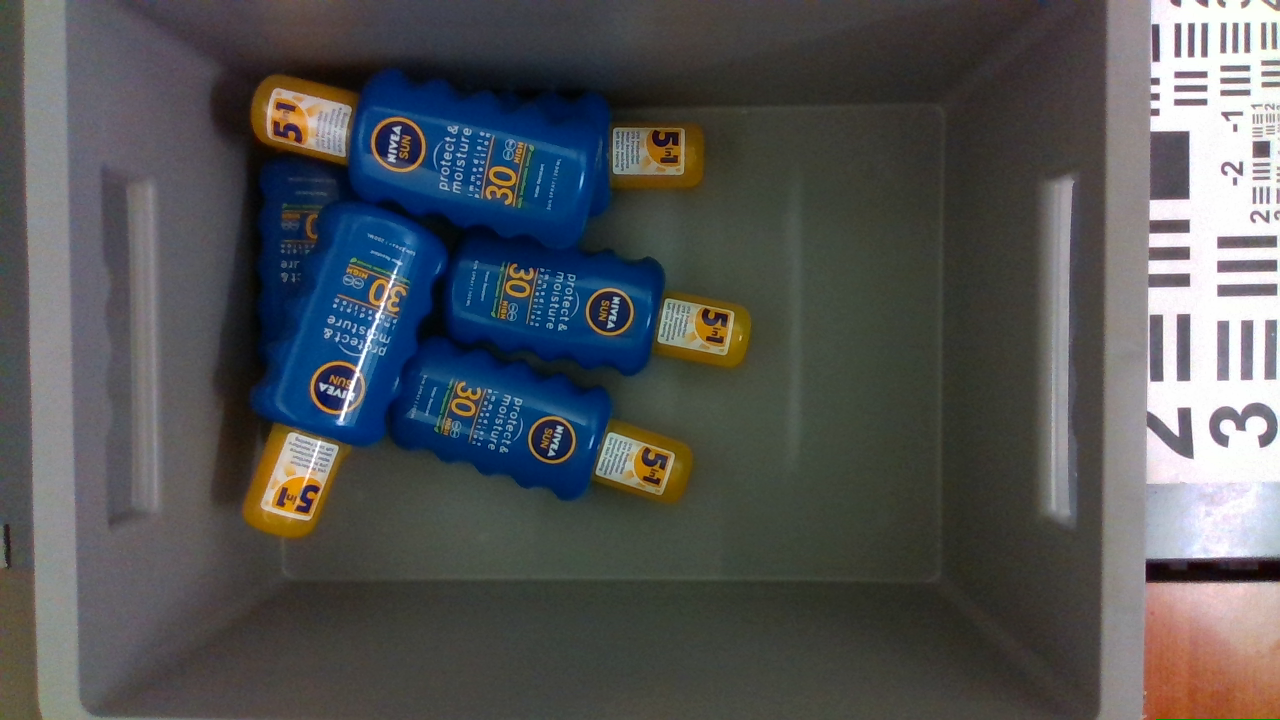
\includegraphics[width=0.2\textwidth]{graphics/beiersdorf/0300.png}}
    \hfill
    \subfloat[Item 4]{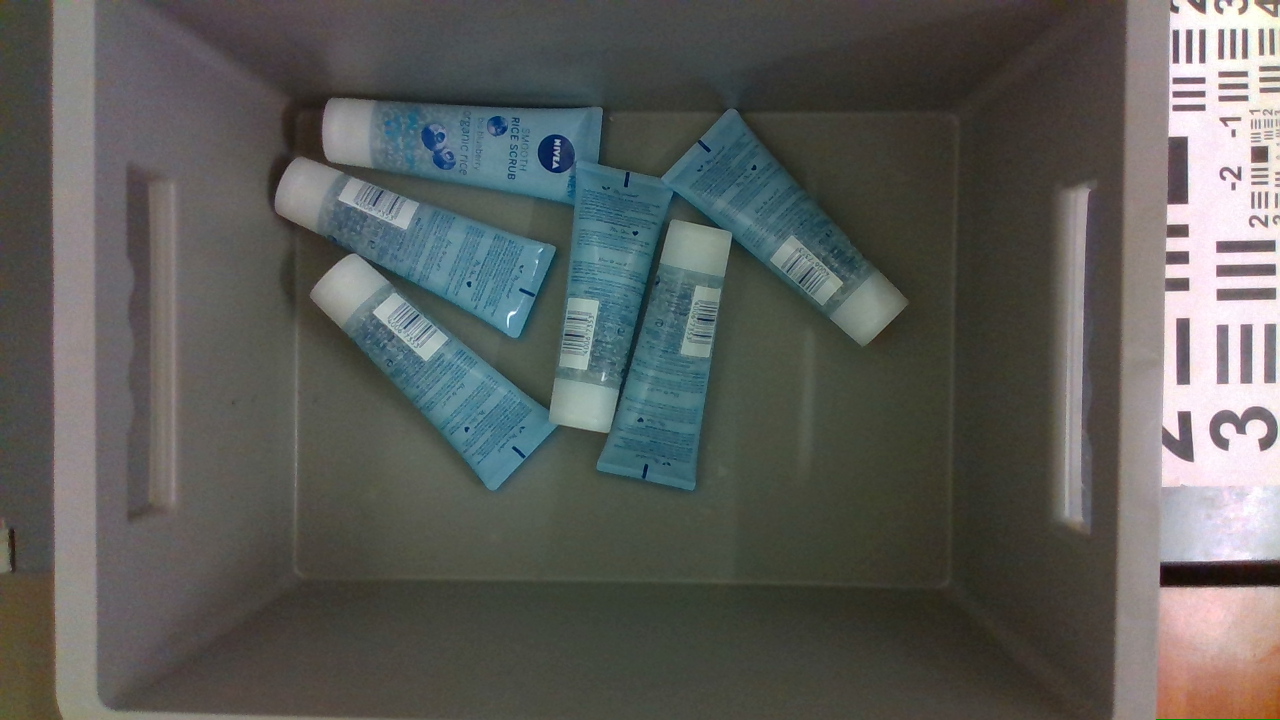
\includegraphics[width=0.2\textwidth]{graphics/beiersdorf/0450.png}}
    \hfill
    \subfloat[Item 5]{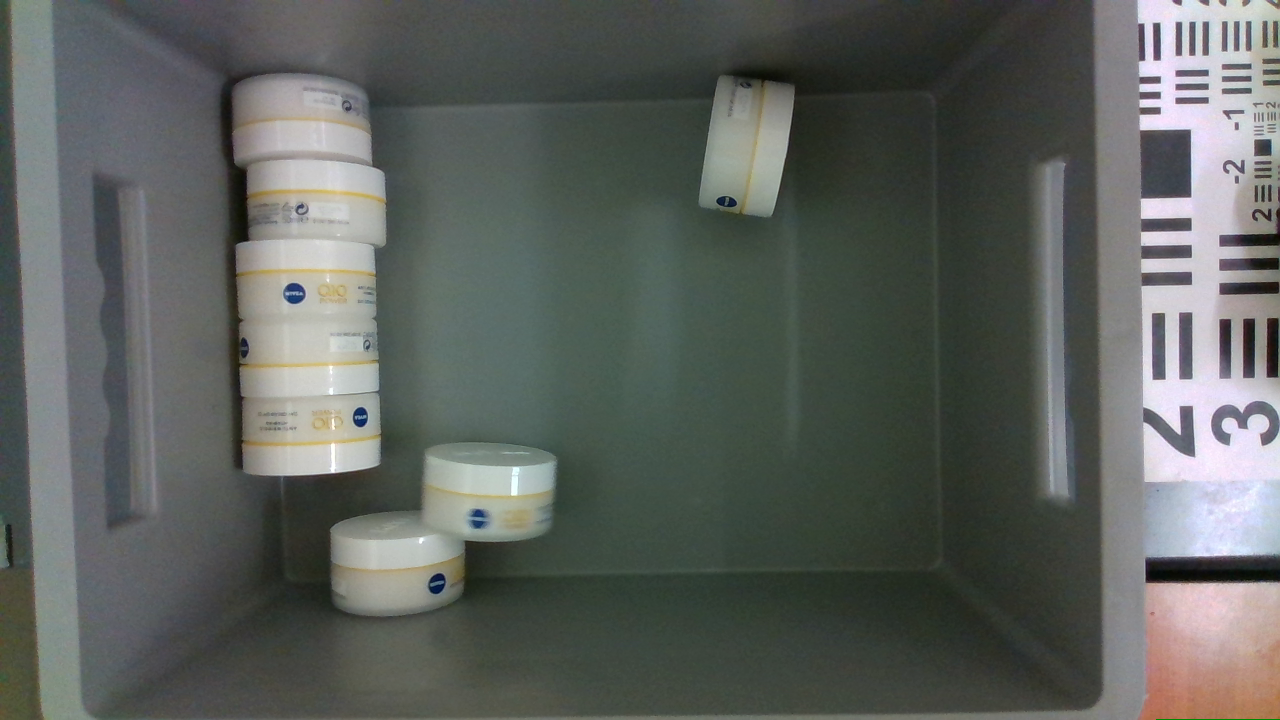
\includegraphics[width=0.2\textwidth]{graphics/beiersdorf/0650.png}}
    \hfill
    \subfloat[Item 6]{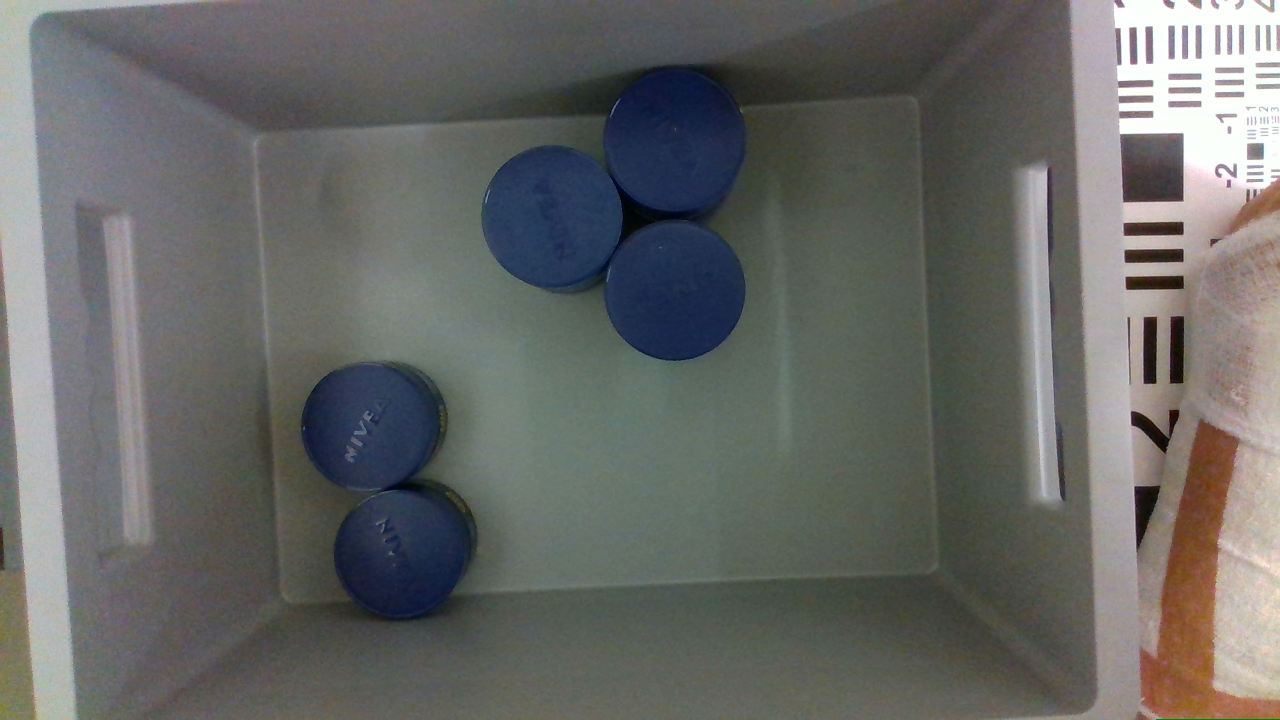
\includegraphics[width=0.2\textwidth]{graphics/beiersdorf/0750.png}}
    \hfill
    \subfloat[Item 7]{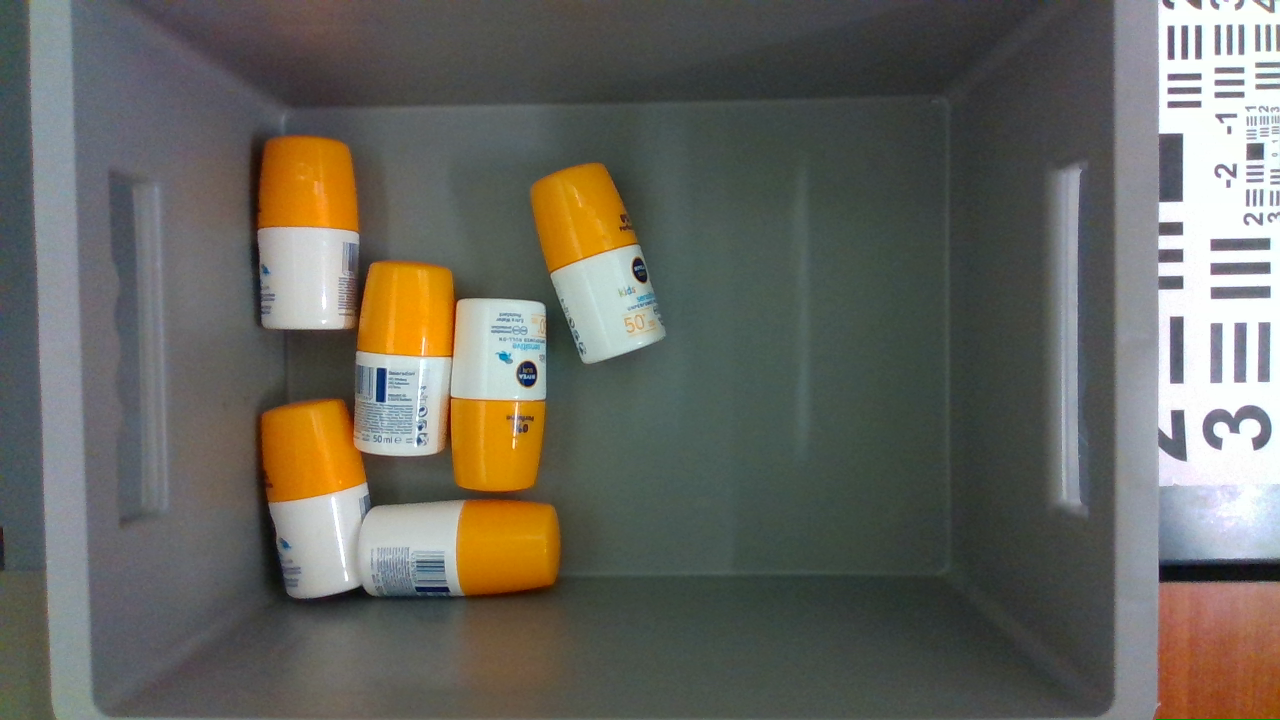
\includegraphics[width=0.2\textwidth]{graphics/beiersdorf/0950.png}}
    \hfill
    \subfloat[Item 8]{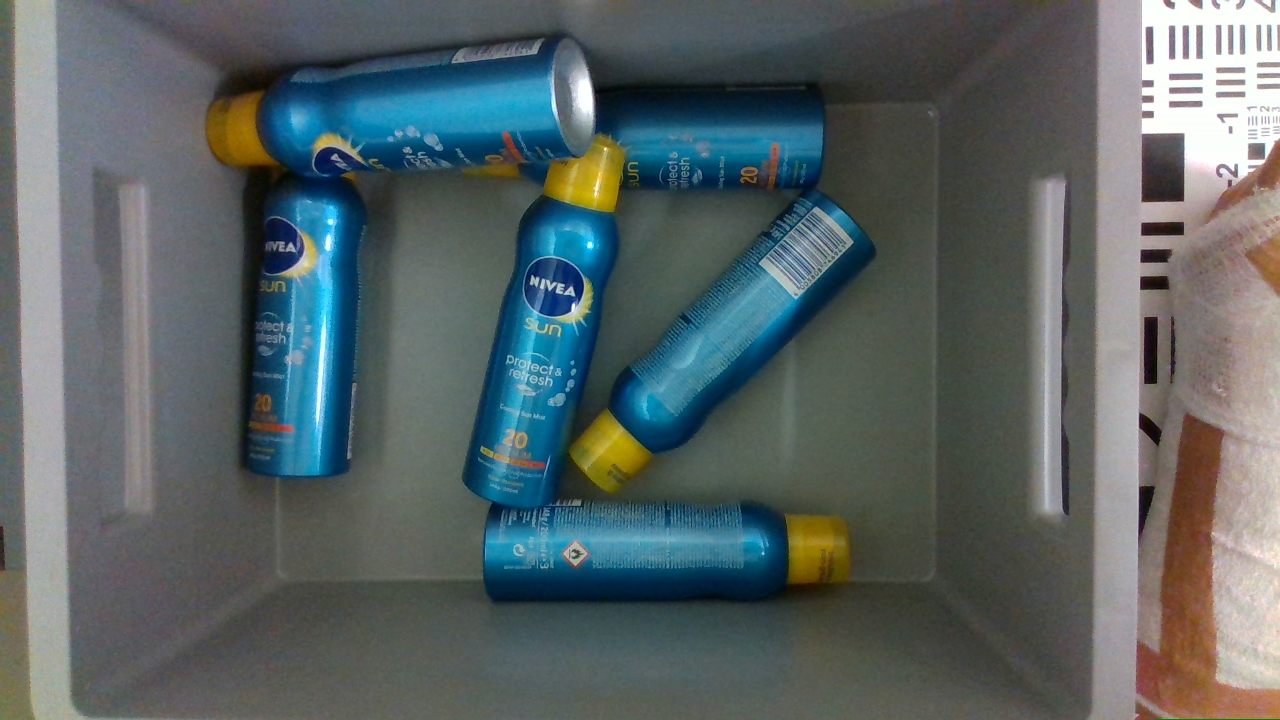
\includegraphics[width=0.2\textwidth]{graphics/beiersdorf/1050.png}}
    \hfill
    \subfloat[Item 9]{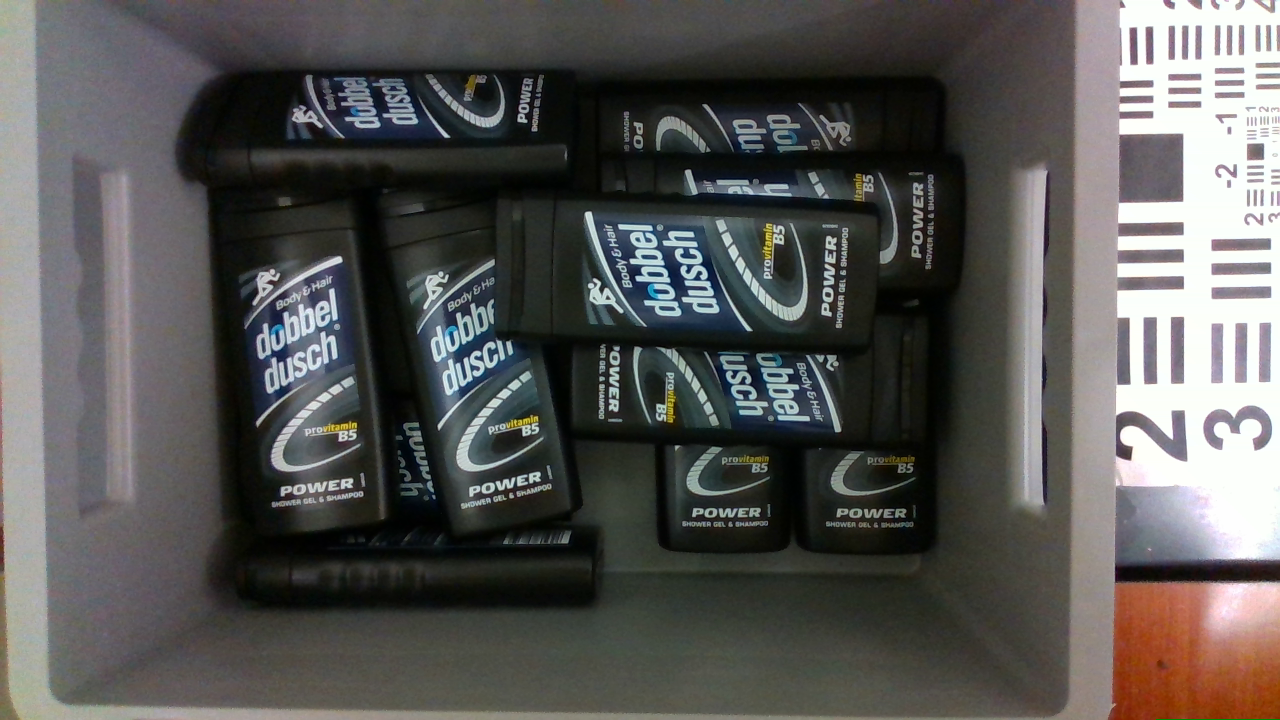
\includegraphics[width=0.2\textwidth]{graphics/beiersdorf/1250.png}}
    \hfill
    \subfloat[Item 10]{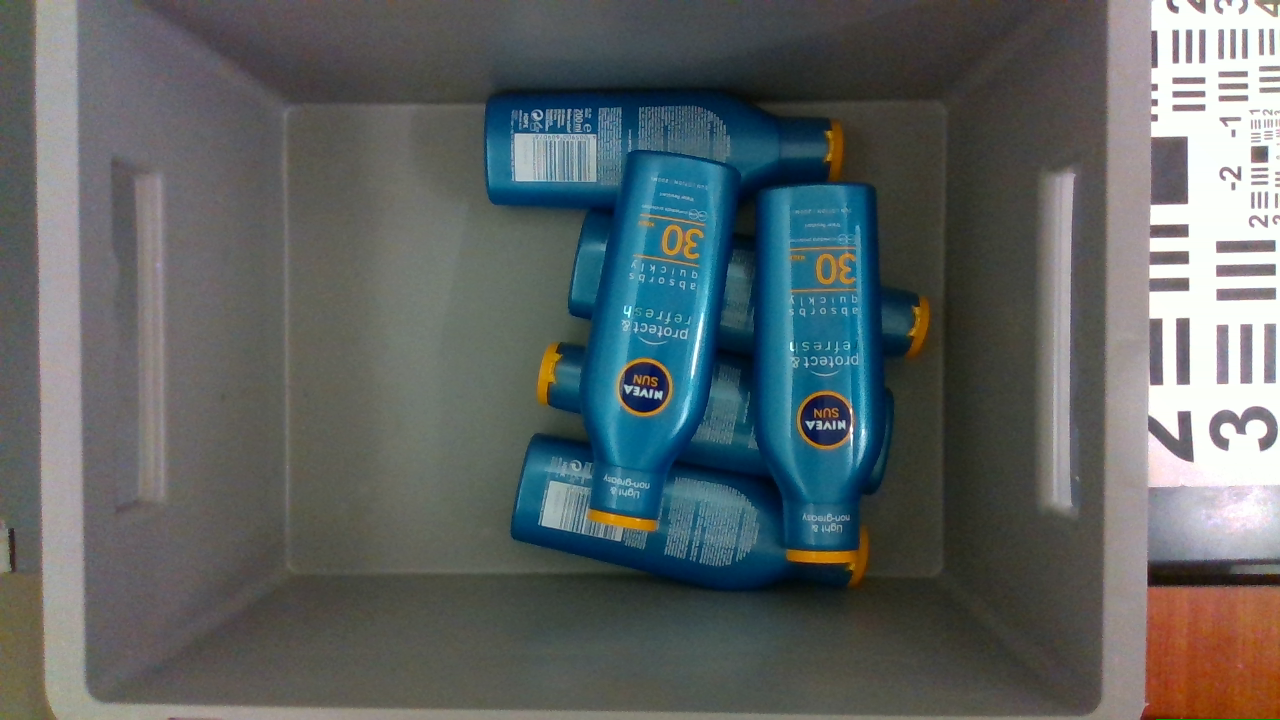
\includegraphics[width=0.2\textwidth]{graphics/beiersdorf/1350.png}}
    \hfill
    \subfloat[Item 11]{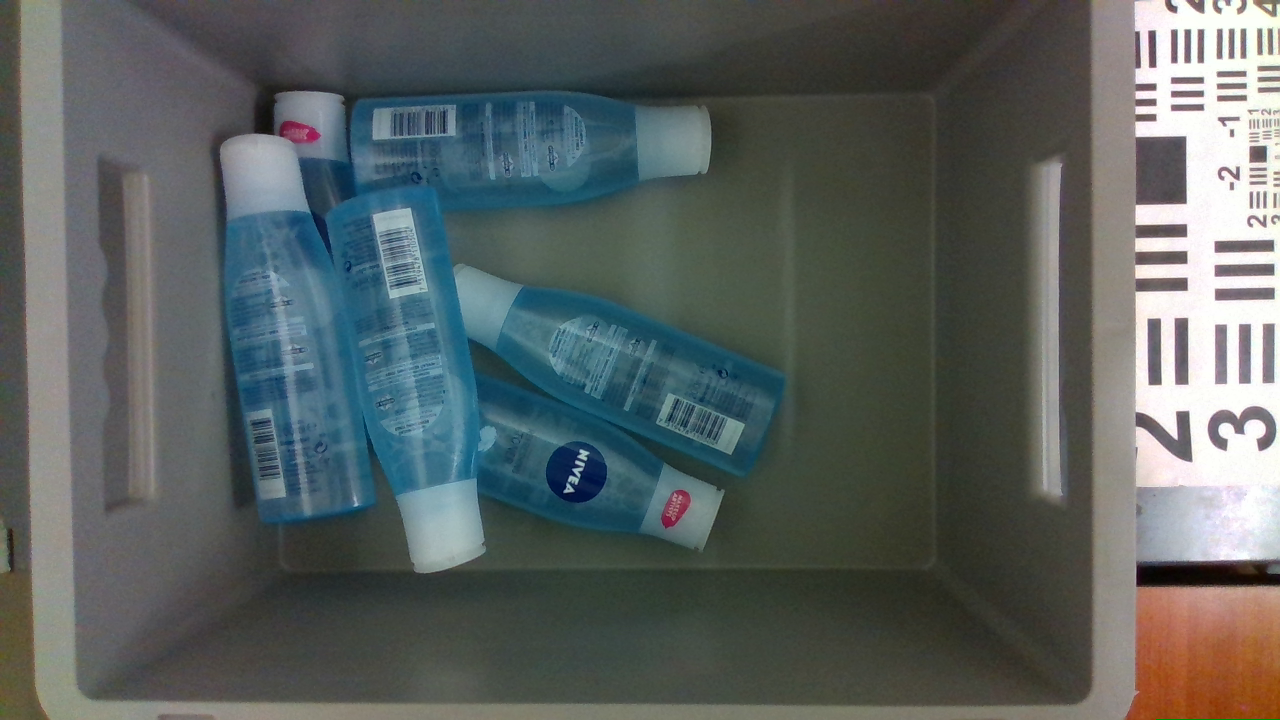
\includegraphics[width=0.2\textwidth]{graphics/beiersdorf/1470.png}}
    \hfill
    \subfloat[Item 12]{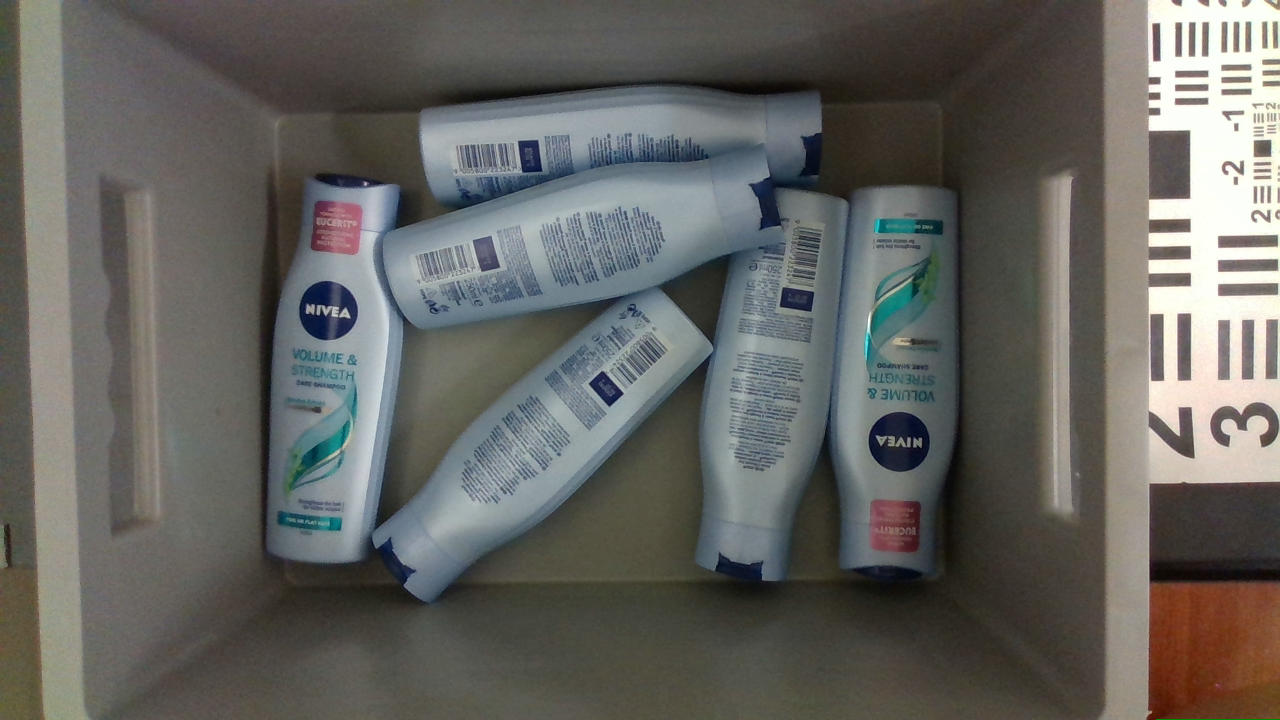
\includegraphics[width=0.2\textwidth]{graphics/beiersdorf/1650.png}}
    \hfill
    \subfloat[Item 13]{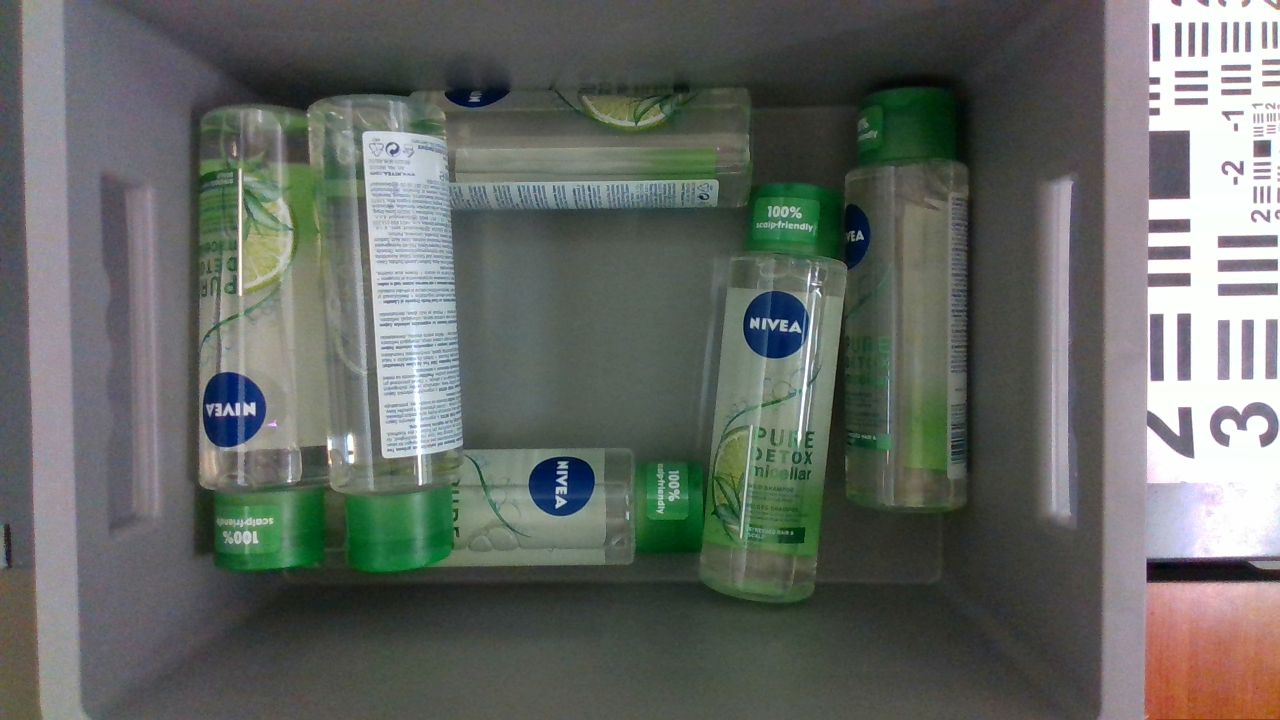
\includegraphics[width=0.2\textwidth]{graphics/beiersdorf/1750.png}}
    \hfill
    \subfloat[Item 14]{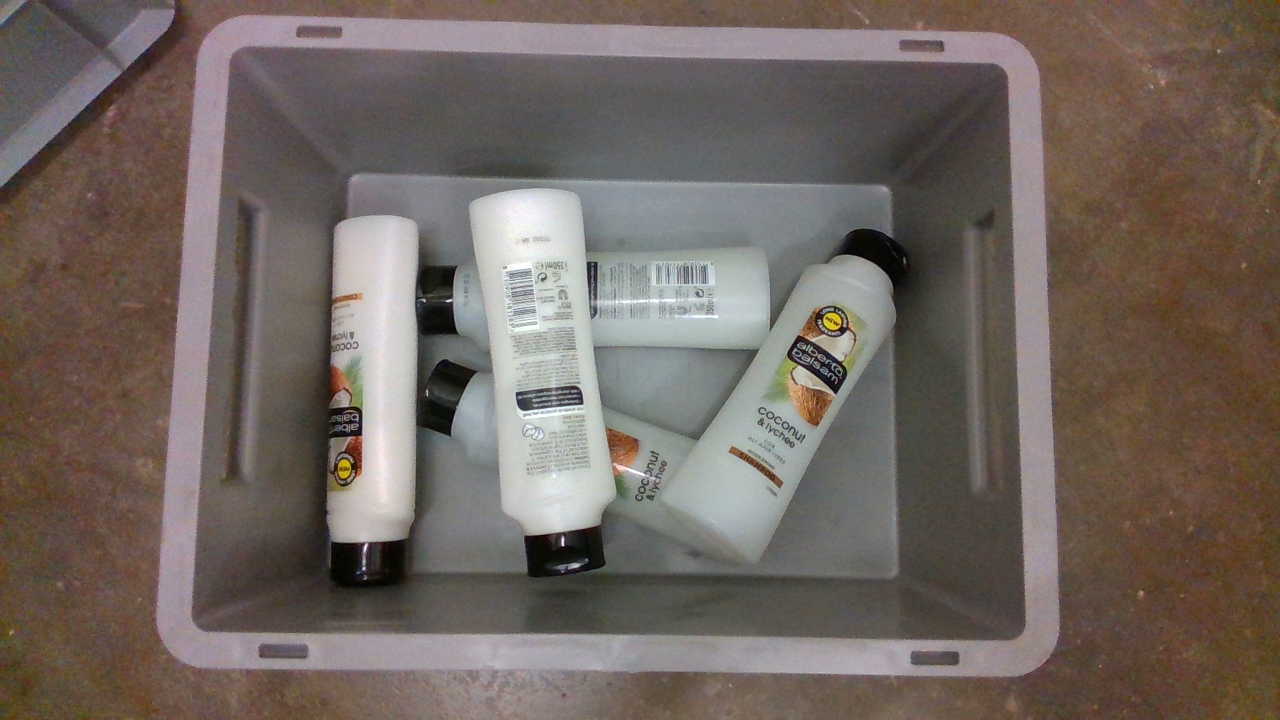
\includegraphics[width=0.2\textwidth]{graphics/beiersdorf/1950.png}}
    \hfill
    \subfloat[Item 15]{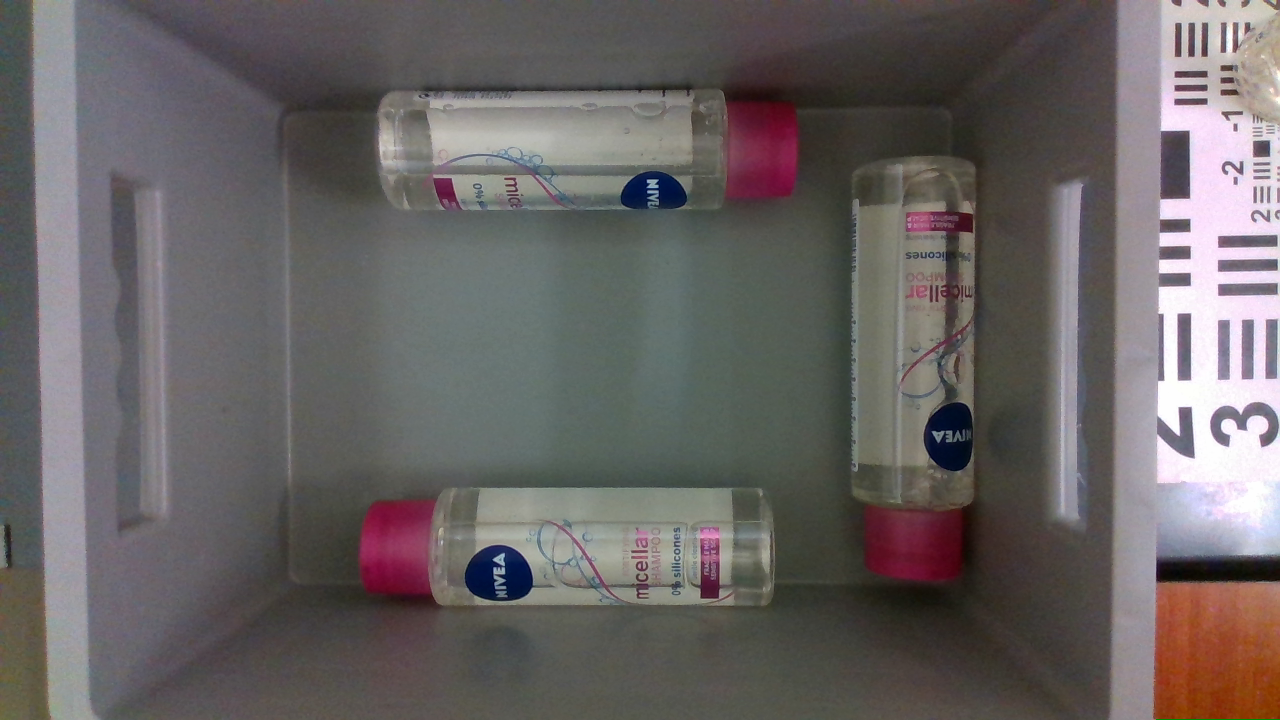
\includegraphics[width=0.2\textwidth]{graphics/beiersdorf/2050.png}}
    \caption{Beiersdorf dataset contains 15 items\cite{bjarnason_1984-_detecting_2021}}
    \label{fig:beiersdorf}
\end{figure}
To be able to use a dataset, it needs to be annotated and the dataset had already been annotated by the former student. It takes 2-10 minutes to annotate an image, averaging approximately 5 minutes per image. When the images are 2175, 10.875 minutes are needed to annotate all the pictures. Which is a lot of manpower for annotating images. \textit{Figure \ref{fig:beiersdorfanno}} below shows how the dataset was annotated with a COCO annotator\cite{brooks_jsbrokscoco-annotator_2021}.
\begin{figure}[h]
    \centering
    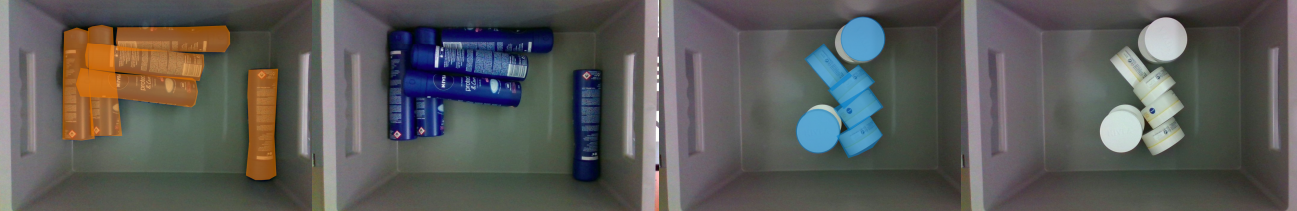
\includegraphics[width=1\textwidth,  angle =0]{graphics/methods/sverrirannotated.PNG}
    \caption{Beiersdorf dataset annotated\cite{bjarnason_1984-_detecting_2021}}
    \label{fig:beiersdorfanno}
\end{figure}

%------------------------------------
\section{Evaluation metrics}
\subsection{Intersection over union}
Intersection over Union (IoU) is known to be a good metric for overlapping two bounding boxes or masks and is used to measure object detector accuracy on a certain dataset. If the estimate is correct, then IoU = 1. The lower the IoU, the worse the results \cite{sheremet_intersection_2020}.

\begin{figure}[h]
    \centering
    % include first image
    \subfloat[An example of a stop sign being detected in a picture. The prediction bounding box is red and the bounding box of the ground-truth is green. ]{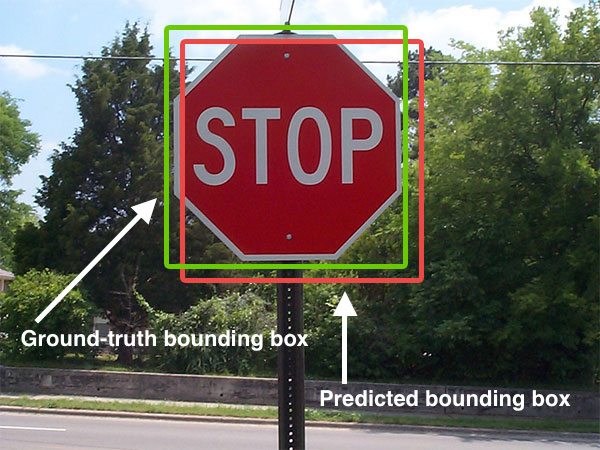
\includegraphics[width=0.48\textwidth]{graphics/iou_stop_sign.jpg}}
    \hfill
    \subfloat[The Intersection of Union are as simple as dividing the overlap zone between boundaries by the union area]{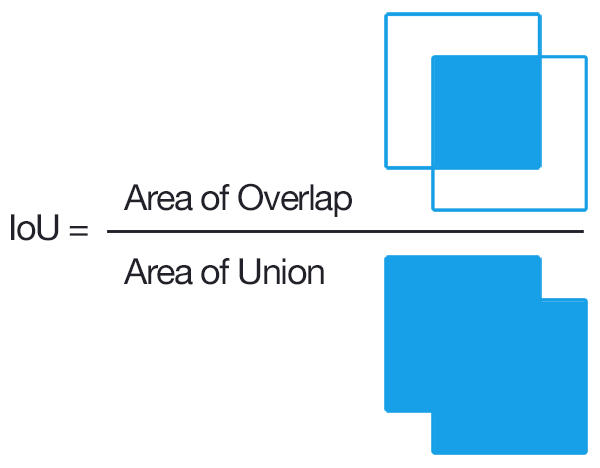
\includegraphics[width=0.48\textwidth]{graphics/iou_equation.png}\label{figure: ioueq}}
    \caption{Intersection over Union for object detection \cite{rosebrock_intersection_2016}}
    \label{figure: iou}
\end{figure}

\begin{equation}
    IoU = \frac{Area\ of\ Overlap}{Area\ of\ Union} \label{eq: ioueq}
\end{equation}
\vspace{0.5cm}

Intersection over Union is simply a ratio between the area of overlap and area of the union when looking at \textit{Equation \ref{eq: ioueq}}.
In the numerator, the area of overlap is calculated between the predicted bounding box and the bounding box.
The denominator is the area of union or, rather, the area covered by both the foreseen boundary and the bottom-wheel boundary\cite{uavs_comparing_2019}.
%\vspace{1cm}
\subsection{Recall, Precision, and F1}
When tests of the performance of the retrieval systems were first developed, an empirical tendency was noticed for recall (completeness) and accuracy (cleanliness of retrieval), both of which appeared to be inversely connected\cite{buckland_relationship_1994}. \textit{Figure \ref{fig:precisionrecall}} explains the precision and recall.



\begin{itemize}
    \item True Positive (TP): The actual positive class is predicted positive.
    \item True Negative (TN): The actual negative class is predicted negative.
    \item False Positive (FP): The actual class is negative but the predicted class is Positive
    \item False Negative (FN): The actual class is positive but the predicted class is negative.
\end{itemize}

\begin{figure}[h]
    \centering
    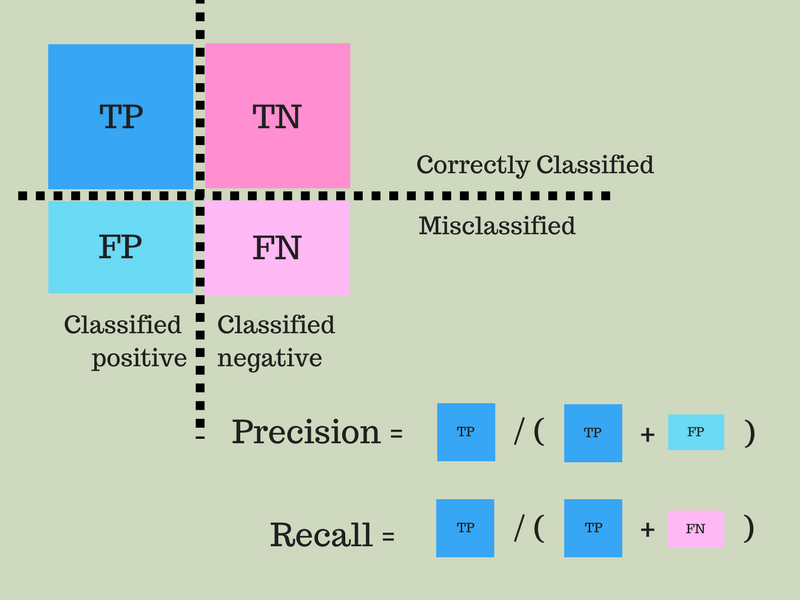
\includegraphics[width=0.8\textwidth]{graphics/Precisionrecall.png}
    \caption{Precision and recall explained \cite{mittapally_whats_2019}}
    \label{fig:precisionrecall}
\end{figure}



Precision is the ratio between the True Positives and all the Positives. In this project, the precision is measured by the number of bottles that we correctly identify out of all the bottles in the bin. It can bee seen in \textit{Equation \ref{eq:precision}}. Precision shows a measure of relevant data points\cite{shung_accuracy_2020}.
\begin{equation}
    Precision = \frac{True\ Positive(TP)}{True\ Positive(TP)+False \ Positive(FP)}
    \label{eq:precision}
\end{equation}


The recall is the measurement of the model that identifies true positives properly. Recall calculates the number of the correct detections divided by the number of actual detections\cite{shung_accuracy_2020}. Recall quantifies the number of positive class predictions made out of all positive examples in the dataset. An example of how recall is calculated can be seen in \textit{Equation \ref{eq:recall}}.
\begin{equation}
    Recall = \frac{True\ Positive(TP)}{True\ Positive(TP)+False \ Negative(FN)}
    \label{eq:recall}
\end{equation}

The F-score is a measure of the precision of a model on a dataset, also known as the F-score. This evaluation is done to evaluate binary classification systems, classifying examples into positive or negative classification systems. 
The F-score combined the precision and recall of the model and is described as the harmonic mean to the precision and recall of the model\cite{wood_f-score_2019}.
An example of how F-score is calculated can be seen in \textit{Equation \ref{eq:f1score}}.
\begin{equation}
    F- score = F_1 = 2 \cdot \frac{Precision \cdot Recall}{Precision + Recall}
    \label{eq:f1score}
\end{equation}


%----------------
\section{Experiment setup}
The best way to automatically annotate objects automatically and see if they will save time and manpower is to perform a few experiments. Those experiments will be explained in more detail in this section.

\subsection{Robot performance}
In this experiment, one test was done on the Franka Emika robot and that was time performance over few iterations. The robot code and how it works is explained in \textit{Section \ref{robotcontrol}}.

In this test, there was only one object in the bin at a time. The time performance was tested on two items \textit{Alberto Balsam} and \textit{Nivea Cleansing Milk}, first with 100 iterations and then with 300 iterations. Which gave us the movement time for one object. In addition, it was checked if the robot needed some help to pick up the item.

\subsection{Automatic labelling performance}
In the automatic labeling experiment, two tests were performed on two methods that were mention in \textit{Sections \ref{beforeandafter} and \ref{emptyvsitem}}. 

One test was performed on the \textit{Before vs After}. That test was simple and was only a visual test executed on the output images, to see the results that method would have.

The other test was performed on the \textit{Empty vs Item in the bin}. That test was executed by a visual test on the output images and also measuring the time that it takes to annotate the images.

\subsection{Trained neural network performance}
Before the automatically labeled dataset got trained it was split into a 75\% train dataset and 25\% test dataset. Then the dataset was trained and three tests were done on the neural network, IoU test, one visually, and an accuracy test(precision, recall, F1-score).


The first test was to measure which epochs model of the neural network would give us the best IoU on the test images. Epochs are the number of times the training set has been presented to the network.

The second test was done by comparing visually before and after results on the neural network. Is the trained neural network better than the original network?

The third test was measuring the accuracy of object detection using a deep neural network trained on the robot-generated data. Measuring the IoU, recall, precision, and F-score and compare it to the results of manual labeling. 